	%%%%%%%%%%%%%%%%%%%%%%%%%%%%%%%%%%%%%%%%%%%%%%%%%%%%%%%%%%%%%%%%%%%%%%%%%%%%%%%%%%%%%%%%%%%%%%%%%%%%%%%%%
	% This template is distribted with ABSOLUTELY NO WARRANTY.
	% It is based on a template from the UT thesis guide (http://web.utk.edu/~thesis/thesisresources.shtml)
	% No claim is made to this intellectual property, since it is based almost entirely on the UT template
%%%%%%%%%%%%%%%%%%%%%%%%%%%%%%%%%%%%%%%%%%%%%%%%%%%%%%%%%%%%%%%%%%%%%%%%%%%%%%%%%%%%%%%%%%%%%%%%%%%%%

	\documentclass[thesis, A4paper, 12pt]{eeeoauthesis} %thesis, one side

	
	\newcommand{\proquestmode}{}
	\newcommand{\bs}{\boldsymbol}
	\renewcommand\bibname{References}
	
	% Set the indentation spacing as well as the paragraph spacing
	\parindent = 0in
	\parskip = 10pt
	%\renewcommand{\baselinestretch}{1.6}
	
	
%%%%%%%%%%%%%%%%%%%%%%%%%%%%%%%%%%%%%%%%%%%%%%%%%%%%%%%%%%%%%%%%%%%%%%%%%%%%%%%%%%%%%%%%%%%%%%%%%%%%%
%%% LOAD SOME USEFUL PACKAGES
%%%%%%%%%%%%%%%%%%%%%%%%%%%%%%%%%%%%%%%%%%%%%%%%%%%%%%%%%%%%%%%%%%%%%%%%%%%%%%%%%%%%%%%%%%%%%%%%%%%%%

\usepackage[stable]{footmisc}           %%%%% stabilizes footnotes that appear in chapters, sections etc.
\usepackage{blkarray}					%%%%% http://ctan.org/pkg/blkarray
\usepackage{graphicx,color}
\usepackage{nomencl}                    %%%%% produces a nomenclature
\usepackage{float}                      %%%%% figure floats          
\usepackage{graphicx}					%%%%% graphics package
\usepackage{fancyhdr}                   %%%%% fancy headers and footers
\usepackage{url}                     %%%%% nicely format url breaks
\usepackage[inactive]{srcltx}		 	%%%%% necessary to use forward and inverse searching in DVI
\usepackage{relsize}                    %%%%% font sizing hierarchy
\linespread2                            %%%%% double lines spacing package
\usepackage{adjustbox}                  %%%%% adjust tables to width of the textmargin
\usepackage{graphicx}
\usepackage{amsmath}
\usepackage{epstopdf}   				%%%%%% allows you to attached eps files	
\usepackage{blkarray} 					%%%%%%% http://ctan.org/pkg/blkarray
\newcommand{\matindex}[1]{\mbox{\scriptsize#1}}  %%%% Matrix index	
\usepackage{booktabs}                   %%%%% professional looking tables
\usepackage[config, labelfont={bf}]{caption,subfig} %%%%% nice sub figures
\usepackage{mathrsfs}                   %%%%% additional math scripts
\usepackage{csquotes}
\usepackage{hyperref}
\makeglossary
\graphicspath{{figures/}{figures/ch2/}{figures/ch3/}{figures/ch4/}{figures/pdf/}}  %%%%%specify the path where figures are located
\usepackage{mfirstuc}
\usepackage{color}
\usepackage[round, sort]{natbib}
%\usepackage{scrextend}
\usepackage{hanging}
\usepackage{titlecaps}
\usepackage{xifthen}
\usepackage[subfigure]{tocloft}
%new from ay
\usepackage{longtable}
\usepackage{geometry}
\usepackage{listings}
\usepackage{xcolor}
\usepackage[vesion=3]{acro}
\usepackage{bigstrut}
%work around to include list of listing to list of figures
\makeatletter
\let\latex@@addcontentsline\addcontentsline
\AtBeginDocument{%
	\renewcommand{\addcontentsline}[3]{%
		\def\@@zzz{#1}\def\@@zxx{lol}
		\latex@@addcontentsline{%
			\ifx\@@zzz\@@zxx lof\else #1\fi
		}{#2}{#3}%
	}

\renewcommand\lstlistingname{Figure}
\let\l@lstlsting\l@figure
\let\c@lstlisting\c@figure
\let\thelstlisting\thefigure
\let\ftype@lstlisting\ftype@figure
}
\makeatother
\newtheorem{dft}{Definition}[chapter]

 
	
%\fancypagestyle{styleempty}{
	\fancyhf{}
%	\setlength{\headwidth}{\textwidth}
%	\addtolength{\headwidth}{\marginparwidth}
%	\addtolength{\headwidth}{\marginparsep}
%	\fancyhead[LE,RO]{\bfseries\thepage}
%	\fancyhead[LO]{\bfseries\rightmark}
%	\fancyhead[RE]{\bfseries\leftmark}
%	\renewcommand{\headrulewidth}{0pt} %<- ADDED
%	\renewcommand{\footrulewidth}{0pt} %<- ADDED%
%}
	
	
	
	
	
%modify chapter here
\usepackage{fmtcount, etoolbox}
%\makeatletter
%\patchcmd{\@makechapterhead}{50\p@}{10pt}{}{}
%\patchcmd{\@makeschapterhead}{50\p@}{10pt}{}{}
%\patchcmd{\@makechapterhead}{40\p@}{20pt}{}{}% Removes space below \chapter head
%\patchcmd{\@makeschapterhead}{40\p@}{20pt}{}{}% Removes space below \chapter* head


\usepackage{titlesec}
\titleformat{\chapter}[display]
{\onehalfspacing \normalfont\bfseries\centering\large}{\MakeUppercase\chaptertitlename\ {\NUMBERstring{chapter}}}{5pt}{\large\MakeUppercase}
%{\singlespacing \normalfont\bfseries\centering\large}{\MakeUppercase\chaptertitlename\ \MakeUppercase\Numberstring{chapter} \thechapter}{5pt}{\large\MakeUppercase}

\titlespacing*{\chapter}
{0pt}{20pt}{30pt}
%\titlespacing*{\section}
%{0pt}{5.5ex plus 1ex minus .2ex}{4.3ex plus .2ex}
%\titlespacing*{\subsection}
%{0pt}{5.5ex plus 1ex minus .2ex}{4.3ex plus .2ex}


%\renewcommand{\cftchapfont}{} 


%\renewcommand{contentsname}{\scshape}
%\renewcommand{cfttoctitlefont}{\centerline{\textbf{\LARGE\sc}}}
\renewcommand{\cfttoctitlefont}{\hspace*{100 pt}\scshape\LARGE}
\renewcommand{\contentsname}{Table of contents}

%\renewcommand{\chapternumberline}[1]{\chaptername\ \numtoName{#1}: }
\renewcommand{\cftchapfont}{\normalfont\scshape} 
\renewcommand *\cftchappresnum {Chapter\ }
\renewcommand{\cftchapaftersnum}{:}
\renewcommand{\cftchapnumwidth}{7em}



\renewcommand{\cftloftitlefont}{\hspace*{130pt}\scshape\LARGE}
\renewcommand{\cftlottitlefont}{\hspace*{130pt}\scshape\LARGE}

\renewcommand\floatpagefraction{0.05}

\fancypagestyle{plain}{%			%redefine Latex plain style so no page number shown
	\renewcommand{\headrulewidth}{0pt}%
	\renewcommand{\footrulewidth}{0pt} %<- ADDED
	\fancyhf{}%
	\fancyfoot{}%
}

	\definecolor{Code}{rgb}{0,0,0}
\definecolor{Decorators}{rgb}{0.5,0.5,0.5}
\definecolor{Numbers}{rgb}{0.5,0,0}
\definecolor{MatchingBrackets}{rgb}{0.25,0.5,0.5}
\definecolor{Keywords}{rgb}{0,0,1}
\definecolor{self}{rgb}{0,0,0}
\definecolor{Strings}{rgb}{0,0.63,0}
\definecolor{Comments}{rgb}{0,0.63,1}
\definecolor{Backquotes}{rgb}{0,0,0}
\definecolor{Classname}{rgb}{0,0,0}
\definecolor{FunctionName}{rgb}{0,0,.7}
\definecolor{Operators}{rgb}{0,0,0}
\definecolor{Background}{rgb}{0.98,0.98,0.98}

\lstdefinestyle{python}{
  numbers=left,
  numberstyle=\footnotesize,
  numbersep=1em,
  xleftmargin=1em,
  framextopmargin=2em,
  framexbottommargin=2em,
  showspaces=false,
  showtabs=false,
  showstringspaces=false,
  frame=l,
  tabsize=4,
  % Basic
  basicstyle=\ttfamily\small\setstretch{1},
  backgroundcolor=\color{Background},
  language=Python,
  % Comments
  commentstyle=\color{Comments}\slshape,
  % Strings
  stringstyle=\color{Strings},
  morecomment=[s][\color{Strings}]{"""}{"""},
  morecomment=[s][\color{Strings}]{'''}{'''},
  % keywords
  morekeywords={import,from,class,def,for,while,if,is,in,elif,else,not,and,or,print,break,continue,return,True,False,None,access,as,,del,except,exec,finally,global,import,lambda,pass,print,raise,try,assert},
  keywordstyle={\color{Keywords}\bfseries},
  % additional keywords
  morekeywords={[2]@invariant},
  keywordstyle={[2]\color{Decorators}\slshape},
  emph={self},
  emphstyle={\color{self}\slshape},
  breaklines=true
}
	
%%%%%%%%%%%%%%%%%%%%%%%%%%%%%%%%%%%%%%%%%%%%%%%%%%%%%%%%%%%%%%%%%%%%%%%%%%%%%%%%%%%%%
%		 TODO: FILL IN YOUR INFORMATION BELOW - READ THIS SECTION CAREFULLY FIRST
% 		 Most of the entries should be in Title Case!
% 		 Replace all "xxxx" with your own data
%%%%%%%%%%%%%%%%%%%%%%%%%%%%%%%%%%%%%%%%%%%%%%%%%%%%%%%%%%%%%%%%%%%%%%%%%%%%%%%%%%%%%
	\title{Design and Development of a Small Scale Bilateral Rehabilitaion Robot for Stroke Rehabilitaion and a low-cost Force-Torque Sensor}	   % Thesis Title. You MUST use correct title case!!! E.g. Development of an Improved Brain Computer Interface
	\authorsurname{Komolafe}   		% Author's surname. E.g Adetayo
	\authorothernames{Elisha Ayobami}   	% Author's other names. E.g Bamidele Judas
	\supervisor{Dr. Kayode Ayodele} 			%Supervisor's title and full name. E.g. Dr. Kayode Ayodele
	\cosupervisor{xxxx} 		%Co-Supervisor's title and full name. E.g. Prof. Morenikeji Komolafe
	
	\supervisorDept{Department of Electronic and Electrical Engineering} 		%supervisor's department. E.g. Department of Electronic and Electrical Engineering
	\cosupervisorDept{xxxx}		%co-supervisor's department e.g. Department of Medicine
	
	\supervisorUni{Obafmi Awolowo University, Ile-Ife} 		%supervisor's university e.g. Obafmi Awolowo University, Ile-Ife
	\cosupervisorUni{xxxx}		%co-supervisor's university
	
	\regnumber{EEG/2015/061}			% registration number e.g. EEG/2017/114
	\thesisyear{2021}			% year of graduation e.g. 2009
	\graduationMonth{December}  	% month of graduation. E.g. June
	\newcommand{\numberOfSupervisors}{1}	% Number of supervisors. Select 1 or 2
	












%%%%%%%%%%%%%%%%%%%%%%%%%%%%%%%%%%%%%%%%%%%%%%%%%%%%%%%%%%%%%%%%%%%%%%%%%%%%%%%%%%%%%
%%%%%%%%%%%%%%%%%%%%%%%%%%%%%%%%%%%%%%%%%%%%%%%%%%%%%%%%%%%%%%%%%%%%%%%%%%%%%%%%%%%%%
%%%%%%%%%%%%%%%%%%%%%%%%%%%%%%%%%%%%%%%%%%%%%%%%%%%%%%%%%%%%%%%%%%%%%%%%%%%%%%%%%%%%%
%%%%%%%%%%%%%%%%%%%%%%%%%%%%%%%%%%%%%%%%%%%%%%%%%%%%%%%%%%%%%%%%%%%%%%%%%%%%%%%%%%%%%
%%%%%%%%%%%%%%%%%%%%%%%%%%%%%%%%%%%%%%%%%%%%%%%%%%%%%%%%%%%%%%%%%%%%%%%%%%%%%%%%%%%%%
%%%%%%%%%%%%%%%%%%%%%%%%%%%%%%%%%%%%%%%%%%%%%%%%%%%%%%%%%%%%%%%%%%%%%%%%%%%%%%%%%%%%%
%		 						!!!!! WARNING  !!!!!
% 		 Do not alter anything from this point downward unless you know what you are
%		 doing. The only reasons you may have to modify anythings below are to 
% 		 (a) add Appendix sections or (b) add one more chapter, which us unlikely
%%%%%%%%%%%%%%%%%%%%%%%%%%%%%%%%%%%%%%%%%%%%%%%%%%%%%%%%%%%%%%%%%%%%%%%%%%%%%%%%%%%%%

%new stuffs
\acsetup{pages/display=none,list/display=used}

\DeclareAcronym{blue}{
short={B.L.U.E.},
long={Bilateral Rehabilitaion Robot},
tag={main}
}
\DeclareAcronym{bluel}{
	short={B.L.U.E.},
	long={Bilateral Rehabilitaion Robot},
	tag={no},
	first-style=long
}
\DeclareAcronym{sz}{
	short={SZ},
	long={Schizophrenia},
	tag={main}
}
\DeclareAcronym{psd}{
	short={PSD},
	long={Power Spectral Density},
	tag={main}
}

\DeclareAcronym{eeg}{
	short={EEG},
	long={Electroencephalogram},
	tag={main}
}
\DeclareAcronym{mmn}{
	short={MMN},
	long={Mismatch Negativity},
	tag={main}
}
\DeclareAcronym{fep}{
	short={FEP},
	long={First Episode Psychosis},
	tag={main}
}
\DeclareAcronym{dsm}{
	short={DSM},
	long={Diagnostic and Statistical Manual of Mental Disorders},
	tag={main}
}
\DeclareAcronym{icd}{
	short={ICD},
	long={International Statistical Classification of Diseases and Related Health Problems},
	tag={main}
}
\DeclareAcronym{mri}{
	short={MRI},
	long={Magnetic Resonance Imaging},
	tag={main}
}

\DeclareAcronym{ct}{
	short={CT},
	long={Computerized Tomography},
	tag={main}
}
\DeclareAcronym{fmri}{
	short={fMRI},
	long={Functional Magnetic Resonance Imaging},
	tag={main}
}
\DeclareAcronym{fnirs}{
	short={fNIRS},
	long={Functional Near Infrared Spectroscopy},
	tag={main}
}
\DeclareAcronym{ssvep}{
	short={SSVEP},
	long={Steady State Visually Evoked Potential},
	tag={main}
}
\DeclareAcronym{p300}{
	short={P300},
	long={300ms Peak Potential},
	tag={main}
}
\DeclareAcronym{n100}{
	short={N100},
	long={100ms Negative Potential},
	tag={main}
}
\DeclareAcronym{erp}{
	short={ERP},
	long={Event Related Potential},
	tag={main}
}
\DeclareAcronym{assr}{
	short={ASSR},
	long={Auditory Steady State Response},
	tag={main}
}
\DeclareAcronym{snhl}{
	short={SNHL},
	long={Sensorineural Hearing Loss},
	tag={main}
}
\DeclareAcronym{gaba}{
	short={GABA},
	long={Gamma-Aminobutyric Acid},
	tag={main}
}
\DeclareAcronym{batrac}{
	short={BATRAC},
	long={Bilateral Arm Training with Rhythmic Cueing},
	tag={main}
}
\DeclareAcronym{arcmime}{
	short={ARCMIME},
	long={ARC Mirror-Image Motion Enabler},
	tag={main}
}
\DeclareAcronym{fma}{
	short={FMA},
	long={Fugl-Meyer Assessment},
	tag={main}
}
\DeclareAcronym{fim}{
	short={FIM},
	long={Functional Independece Measure},
	tag={main}
}
\DeclareAcronym{mss}{
	short={MSS},
	long={Motor Status Score},
	tag={main}
}
\DeclareAcronym{dof}{
	short={DOF},
	long={Degree's of Freedom},
	tag={main}
}
\DeclareAcronym{ct}{
	short={CT},
	long={Computerized Tomography},
	tag={main}
}
\DeclareAcronym{mri}{
	short={MRI},
	long={Magnetic Resonance Imaging},
	tag={main}
}
\DeclareAcronym{eeg}{
	short={EEG},
	long={Electroencephalogram},
	tag={main}
}
\DeclareAcronym{ecg}{
	short={ECG},
	long={Electrocadiagram},
	tag={main}
}
\DeclareAcronym{built}{
	short={BUiLT},
	long={Bilateral Upper Limb Trainer},
	tag={main}
}
\DeclareAcronym{vr}{
	short={VR},
	long={Virtual Reality},
	tag={main}
}
\DeclareAcronym{dmct}{
	short={DMCT},
	long={Dose Matched Control Training},
	tag={main}
}
\DeclareAcronym{mcimt}{
	short={mCIMT},
	long={Modified Constraint-Induced Movement Therapy},
	tag={main}
}
\DeclareAcronym{mbatrac}{
	short={mBATRAC},
	long={Modified Bilateral Arm Training with Rhythmic Cueing},
	tag={main}
}
\DeclareAcronym{cimt}{
	short={CIMT},
	long={Constraint-Induced Movement Therapy},
	tag={main}
}
\DeclareAcronym{ultra}{
	short={ULTRA},
	long={Upper Limb TRaining After stroke},
	tag={main}
}
\DeclareAcronym{semg}{
	short={sEMG},
	long={surface Electromyograms},
	tag={main}
}
\DeclareAcronym{wmft}{
	short={WMFT},
	long={Wolf Motor Function Test},
	tag={main}
}
\DeclareAcronym{mas}{
	short={MAS},
	long={Modified Ashwort Score},
	tag={main}
}
\DeclareAcronym{ulexo}{
	short={EXO-UL7},
	long={7 \acs{dof} Upper Limb Exoskelton Robot},
	tag={main}
}
\DeclareAcronym{ul}{
	short={UL},
	long={Upper Limb},
	tag={main}
}
\DeclareAcronym{arm}{
	short={ARM},
	long={Assisted Rehabilitation and Measurement},
	tag={main}
}
\DeclareAcronym{ipam}{
	short={iPAM},
	long={intelligent Pneumatic Arm Movement},
	tag={main}
}
\DeclareAcronym{nere}{
	short={NeReBot},
	long={Neuro-Rehabilitation Robot},
	tag={main}
}
\DeclareAcronym{bmt}{
	short={BMT},
	long={Bi-Manu Track},
	tag={main}
}
\DeclareAcronym{rd}{
	short={RD},
	long={Rhea-Digit},
	tag={main}
}
\DeclareAcronym{rsd}{
	short={RSD},
	long={Rhea-Slide-Due},
	tag={main}
}
\DeclareAcronym{rs}{
	short={RS},
	long={Rhea-Slide},
	tag={main}
}
\DeclareAcronym{pd}{
	short={PD},
	long={Propotional Derivative},
	tag={main}
}
\DeclareAcronym{cvs}{
	short={CVS},
	long={Cardiovascular System},
	tag={main}
}
\DeclareAcronym{fsr}{
	short={FSR},
	long={Force Sensing Resistors},
	tag={main}
}
\DeclareAcronym{pulsr}{
	short={PULSR},
	long={Platfor for Upper Limb Stroke Rehabilitation},
	tag={main}
}
\DeclareAcronym{eoa}{
	short={EOA},
	long={End-of-Arm Tooling},
	tag={main}
}
\DeclareAcronym{ur}{
	short={UR},
	long={Universal Robots},
	tag={main}
}
\DeclareAcronym{id}{
	short={text},
	long={text},
	tag={main}
}





























































































	\begin{document}  	   	
	   	
		%\pagenumbering{alph} 	 
		
		\addToPDFBookmarks{0}{Front Matter}{rootNode} 		
		\addToPDFBookmarks{1}{Title}{a}  					
		\makeTitlePage 			
		 
		 		 
		\pagenumbering{roman}
		\setcounter{page}{1}	
		
		\addToPDFBookmarks{1}{AuthorizationPage}{a} 
		\makeAuthorizationPage 
		
		\addToPDFBookmarks{1}{CertificationPage}{b} 
		\makeCertificationPage{\numberOfSupervisors}	
		
		\addToPDFBookmarks{1}{Acknowledgements}{c} %%%add a pdf bookmark to the acknowledgements page
		\chapter*{ \textbf{\Large \sc Acknowledgements}}
\vspace{50pt}


% TODO : Write the text of your acknowledgement below, using proper Latex syntax.

xxxx %%%include the acknowledgements	
		 
		\addToPDFBookmarks{1}{Dedication}{d} %%%add a pdf bookmark to the dedication page
		\chapter*{ \textbf{\Large \sc Dedication}}
\vspace{50pt}

% TODO : Replace the text "xxxx" below with your dedication.



\begin{center}
{\centering \it To my family(mother and sisters) for their patience, to my supervisor for his unflinching support and patience, and to God for the gift of knowledge, wisdom and choice.}
\end{center} %%%include the dedication
		 
		\begin{spacing}{1.5}  		
			\addToPDFBookmarks{0}{Table of Contents}{e}
			\tableofcontents %generate a table of contents		
			 
			\addToTOC{List of Figures} %%%this will add the list of figures to the Table of Contents (TOC)
			\listoffigures %%%%%generate a list of figures		
			
			\addToTOC{List of Tables} %%%this will add the list of tables to the Table of Contents (TOC)
			\listoftables % generate a list of tables
		\end{spacing}
			
			
		\addToPDFBookmarks{1}{Abbreviations}{f} 
		\addToTOC {List of Abbreviations}
		%\include{front-matter/Abbreviations} %%%List of Acronyms   %%%%%%%%%%%%%	
	
		\printacronyms[name={ \textbf{\Large \sc List of Abbreviations}},include={main}]
		 
		\addToPDFBookmarks{1}{Abstract}{g} %%%add a pdf bookmark to the abstract page
		\addToTOC {Abstract}
		\include{front-matter/Abstract} %%%abstract		 
		 
		 
		 
		%%%%%%%%%%%%%%%%%%%%%%%%%%%%%%%%%%  set page numbering at the top of the page here
	 	%\newpage
		\pagenumbering{arabic}
		\setcounter{page}{1}  

		\fancyhf{}
		\fancyfoot[C]{\thepage}
		\thispagestyle{plain}
		\pagestyle{fancy}
		\renewcommand{\headrulewidth}{0pt}%
		\renewcommand{\footrulewidth}{0pt} %<- ADDED	
	
		%%%%%%%%%%%%%%%%%%%%%%%% TODO: INCLUDE THE CHAPTERS STARTING WITH THE NOMENCLATURE IF PRESENT %%%%%%%%%%%%%%% 
		\chapter{Introduction}\label{Ch:1}		% TODO: you can change the chapter title from Introduction if necessary

\section{Background}\label{sec:Intro}	
\ac{sz} is a brain disorder characterised by recurrent or continuous psychotic episodes (an altered view of reality) marked by 
auditory, visual, and delusional hallucinations, in addition to many other characteristics that are typical of \ac{sz} populations. 
Some other symptoms include consistent disorganised thinking, social withdrawal, decreased emotional expression and apathy. \ac{sz} is 
seen as an hetrogeneous syndrome and often referredto as a multitude of disease states\cite{bakhshi2015neuropathology}.

Statistics from 2011 indicate that there are 21 million people with \ac{sz} worldwide (about one of every 285). Data from the 
previous 50 years also demonstrates \ac{sz}'s comparatively steady occurrence throughout time. \ac{sz} is diagnosed in men 
1.4 times more frequently than in women, and it typically manifests in men earlier. Males typically experience psychosis at ages 20 to 
28 and females typically experience it at ages 26 to 32. Before the age of 13 and between the ages of 40 and 60, early and late onsets 
of psychosis are possible. The average age of patients being treated for \ac{sz} in hospitals is from 25 to 35 years old. The 
Middle East and East Asia have the highest populations of \ac{sz} worldwide, with the western and certain northern regions of 
Africa having the highest prevalence.

In its early phases, \ac{sz} is dormant and only gets worse with time. \ac{fep} is the pivotal point in the 
epidemiology of a \ac{sz} case; in the prodromal phase (pre-psychosis), it is initially asymptomatic (without noticeable symptoms), 
and it is only diagnosed after the \ac{fep}, which often occurs in adolescence or young adulthood. Positive, negative, or cognitive symptoms 
are all categories used to describe \ac{sz}. The cognitive symptoms are seen following \ac{fep} during mental tasks like arithmetic 
problems or difficult essay readings. The cognitive symptoms are less evident compared to the positive and negative symptoms in typical 
day-to-day activities. It can be challenging to make a diagnosis of \ac{sz} before \ac{fep} because these symptoms are frequently 
transitory and dormant before \ac{fep}.

Positive signs of psychosis include delusions, hallucinations, disorganised speech and thinking, and other types of altered responses and 
behaviour. Only after psychosis are the positive symptoms visible. 80\% of people with \ac{sz} experience hallucinations, which 
are largely related to auditory processes. The auditory hallucinations are a sign of a impaired auditory cortex (brain area responsible 
for auditory processes) functioning. The severity of hallucinations varies amongst individuals based on the number of sensory organs implicated and 
the degree of brain pathways linked to those sensory organs that are impaired. Passivity phenomenon, in which the patient feels that an 
outside force is influencing or controlling his or her thoughts and activities, is another helpful sign of \ac{sz}. Positive 
symptoms improve with treatment and lessen as the illness progresses.

Negative symptoms are impairments in regular emotional reactions or in other mental processes connected to feelings. Flat expressions or 
little emotion (blunt affect), poor speech (alogia), an inability to feel pleasure (asociality), a lack of desire to develop 
relationships (avolition), a lack of motivation, and apathy are some of the negative symptoms that have been discovered. Negative 
symptoms are rarely observed because they are indiscriminate and unique to each individual. Since they are tethered to human emotion, 
it is challenging to draw judgments about them only from their traits. Avolition and anhedonia are signs of a brain circuitry problem 
with reward processing which is associated with the prefrontal cortex of the brain. As a component of the brain's reward circuitry, the dorsal prefrontal cortex, brain signals from this region can shed light on how the reward circuitry differs in \ac{sz} populations and non \ac{sz} groups. Most \ac{sz} cases of negative symptoms are  associated with apathy and  are related to disrupted cognitive processing affecting memory and planning including goal directed-behaviour. 
Secondary negative symptoms are those that develop as a result of primary positive symptoms, antipsychotic drug side effects, substance 
use disorder, and social isolation, while primary negative symptoms are those that are innate to \ac{sz}. Compared to the original 
negative symptoms, the secondary negative symptoms are significantly more responsive to treatment. Negative symptoms are sometimes 
mistaken for hormonal fluctuations or stages of social disobedience, especially in adolescence, and are thus readily disregarded in 
day-to-day activities.

70\% of people with \ac{sz} experience cognitive symptoms, which are more pronounced and recurrent in both early and late stages 
of the illness. The existence and severity of cognitive dysfunction are seen as greater indicators of functionality than the presentation 
of core symptoms, despite the fact that they are not considered to be core symptoms of \ac{sz}. Cognitive deficiencies worsen 
during the initial psychotic episode, then recover to normal and stay largely stable throughout the disease. Social or non-social 
cognitive deficiencies are also possible. In populations with \ac{sz}, the following cognitive abilities are frequently accessed: verbal fluency, knowledge retention capacity, reasoning, problem-solving, processing speed, auditory perception, and visual perception. The most noticeable impairments are 
in verbal memory and attention, which all indicate damaged neural networks in the brain and altered brain function (reaction) to inputs. Cognitive impairment is also linked to episodic memory and visual backward masking. Antipsychotic medications have no effect on cognitive deficits; therapy is the preferred method of treatment.

Due to its difficult diagnosis, complex character, and concomitant post-psychotic behaviour symptomatic nature, which is mostly a 
combination of the behavioural symptoms of a significant class of mental diseases, \ac{sz} has been referred to as the heartland of 
psychiatry \cite{goodwin2007heartland}. \ac{sz} has no precise boundary spreading its psychotic manifestations across that of other 
mental disorders and its exact causation is unknown, for this reason, \ac{sz} is seen as an interplay of different factors causing 
multiple mental disorders occurring simultaneously and this also makes it difficult to identify \ac{sz} cases even after \ac{fep}. It 
is also hypothesised that it results from a complex interaction between genetic and environmental risk factors that affect early brain 
development and the course of biological adaptation to experiences in life. Of all hypothesised causative factors of \ac{sz}, the genetic and 
environmental factors have been more prevalent in cases of \ac{sz} and genetics hypothetically accounts for an estimated value of 
between 70\% and 80\% of \ac{sz} cases. However, \cite{etiologySZ} show that most people with \ac{sz} have no family history of psychosis. Also results of 
candidate gene studies have generally failed to find consistent associations. The question of how \ac{sz} could be primarily 
genetically influenced, given that \ac{sz} populations have lower fertility rates remains a paradox. However, consistently, the gene-loci 
explained by genome-wide association studies explains only a small fraction of the variations in \ac{sz}. This reduces the confidence level 
in using genetic factors in prediction of \ac{sz} remission, epidemiology of \ac{sz} and identification of \ac{sz} risk population.

Genetic and environmental biomarkers of \ac{sz} have produced inconsistent results in multiple works, thus existing methods of identifying \ac{sz} require some level of active psychosis so as to take advantage of positive and negative symptoms  and  generates behavioural information for psychiatric evaluation based on some psychiatric criteria such as the \ac{dsm} or the \ac{icd}. Very little empirical data such as \ac{mri} or \ac{ct} scan is used in identifying \ac{sz} and quality of psychiatric evaluation is subject to the experience and competence of the mental health official. Methods of treatment vary from patient to patient and after psychosis, is usually an individually tailored combination of talking therapy and medicine which is a very expensive process and mostly lifelong. \ac{sz} can be treated and managed if discovered early, before the onset of psychosis, but the pre-psychosis non salient nature of its symptoms make early identification, thus prevention difficult and the cost of treatment after \ac{fep} is high for the average worker accounting for the cost of therapy, antipsychotics, electroconvulsive therapy, hospitalisation and other processes. In the use of psychiatric evaluation methods the need of psychosis indicates already active \ac{sz} which is a mental condition that is best prevented as its treatment can be lifelong and similar talking therapy and medicine can prevent transition into psychosis. For these reasons, there is the need to develop a standard empirical test for identification of \ac{sz} risk population and active \ac{sz} patients.

Research works done on identifying the pathophysiology of \ac{sz} have produced results which are not generic to a significant percentage of the \ac{sz} population with inconsistencies in results employing the same approach. This may be due to the comorbid nature of mental-disorders in \ac{sz} patients, the variations in genetic material behaviour among patients, the dynamism of brain networks among patients and so many other factors. Also the symptoms of \ac{sz} can only be utilised after \ac{fep}. Research has not been able to establish a specific cause of the comorbid nature of \ac{sz} and thus has not been able to establish a particular factor as the primary agent responsible for \ac{sz}. Seeking for answers at the cell/tissue level of organisation seems to be a longshot, therefore, can higher levels of human biological organisation (organ/system) provide early diagnostic methods of \ac{sz} risk populations and \ac{sz} patients. This brings us to the study of the neuronal, brain and cortical structures of the brain, their characteristics, functions and how \ac{sz} alters their behaviour.

Based on the fact that prodromal and post-psychotic stages of \ac{sz} are consistently accompanied by an evolution (degradation) of brain information processing in schizophrenic populations, perhaps in developing an empirical test for \ac{sz} (characterising \ac{sz} patients and establishing links between genetic risk, brain biology, and other suspected factors), research should look beyond the symptoms and investigate the brain processes that result in these symptoms. As stated before, positive symptoms(hallucinations, delusions) indicate impaired auditory, visual and other sensory neural pathway functions in the brain, negative symptoms(apathy and social interaction) indicate impaired prefrontal cortex and other brain regions that act as seats of, or interact with emotional intelligence processing and also, cognitive symptoms indicate neural pathways responsible for cognitive functions are impaired some of which are found in the cerebral cortex and frontal cortex. Brain signals acquisition methods, such as the \ac{fep}, \ac{fmri}, \ac{fnirs}, are usually reflective of these changes. Research work done overtime has shown that some of these brain signal acquisition methods have given consistent results in discriminating between \ac{sz} patients, risk population and  non-\ac{sz} population. Some research also shows some of these successfully predict remission from \ac{sz} and predict the path taken by \ac{sz} towards or away from remission. Among the stated methods we will describe and focus on the non-invasive \ac{eeg}.
\subsection{Electroencephalography and Schizophtrenia}
The non-invasive \ac{eeg} is a method of acquiring electrical signals of the brain, which requires no surgical procedure. Signals from non-invasive \ac{eeg} are used to study the brain, understand its cortical level of organisation, study changes in cortical behaviour in response to events and in case of diseases and ailments. \ac{eeg} systems are preferred in most research works because of the balance between cost and quality of signal acquired in terms of temporal and spatial resolution. \ac{eeg} offers fine temporal resolution over spatial resolution, which is usually compensated for by the use of increased number of electrodes. In any study involving \ac{eeg} signals, certain signal classes are monitored in the frequency domain and certain time-domain behaviour is monitored. In the frequency domain, interested frequencies of oscillations are usually the beta(12-30Hz) for activities of motion and gamma(30Hz and above) for cognitive functions. Study of time-domain changes are usually attached to response to stimulus events, visual, auditory or somatosensory. Some time domain signal behaviours include \ac{p300}, \ac{n100}, \ac{mmn} and many more. And in certain cases the time-frequency domain gives information, a typical example being the \ac{ssvep}. \ac{eeg} based methods of identification of \ac{sz} patients and prediction of path of \ac{sz} evolution has provided consistent and statistically significant results over the years, which show that increased study of the \ac{eeg} signal classes in \ac{sz} and non \ac{sz} population will eventually lead to the development of a point of care, prognostic tool for \ac{sz}.

In light of the existence of auditory, visual and somatosensory hallucinations in \ac{sz} patients, impaired cognitive and social function, certain \ac{fep} signal classes that are indicative of the state of these functions have been found to be consistently altered in the \ac{sz} patients and risk population. One prominent class is the mismatch negativity which occurs in response to auditory and visual stimuli. The mismatch negativity (\ac{mmn}) is a component of the brain \ac{erp} to an odd stimulus in a sequence of stimuli. The \ac{mmn} signal occurs due to sudden change in parameters of the stimuli, such as frequency of sound within a standard time, time duration of signal of a standard frequency, sudden change in gradient of light intensity, etc. The \ac{mmn} signal is consistently attenuated in \ac{sz} at risk populations and \ac{sz} patients. Another class of \ac{fep} signal is the \ac{assr}. \ac{assr} is evoked using repeated sound stimuli presented at a high repetition rate and can be used to objectively estimate hearing sensitivity in individuals with normal hearing sensitivity and with various degrees and configurations of \ac{snhl}. \ac{sz} patients consistently show reduced \ac{assr} power and phase locking to gamma range stimulation. Since \ac{fep} results are significantly consistent in \ac{sz} patients and risk population,  how can they be used in developing a point of care prognostic measures for \ac{sz}.

\subsection{Problem Description}
In the quest of developing empirical methods of characterising \ac{sz} patients and discrimination \ac{sz} risk population from the non \ac{sz} populace, the medical and biological sciences seem to have hit a gridlock in seeking for pathological, environmental and genetic causes of \ac{sz} that consistently characterize \ac{sz} behaviour and its prognosis. In areas of genetics, inconsistencies have been found in the results of various research modalities. The comorbid nature of the \ac{sz} condition also makes it difficult to identify pathological causes of \ac{sz} and there exists limitations on social methods of determining environmental factors and causes of \ac{sz}, as these social methods may not be empirical enough to reach a conclusion.

\ac{eeg} methods of identifying \ac{sz} affected and risk population have provided more consistent results and has helped understand the ailment and develop various models that explained the ailment to an extent, one of such being the functional connectivity model which suggest reduced level of interaction between brain  regions. The functional connectivity model has shown that people with \ac{sz} show both higher diversity at each brain region and lower variance in connectivity strength across the brain. This can be conceptualised as a randomization or de-differentiation of functional connectivity.

\ac{eeg} methods have also suggested the use of auditory sensitive \ac{erp}'s in identifying \ac{sz} affected and risk populations. As stated before, the \ac{mmn} is a prominent \ac{erp} in \ac{fep} studies of \ac{sz}. The \ac{mmn} is consistently attenuated in \ac{sz} populace and has some other \ac{erp} components that are concomitant to it and altered in \ac{sz} patients. One such \ac{erp} is the P3a. Auditory P3a response is a fronto-centrally maximal positive component elicited by infrequent, unpredictable stimuli in a stream of repeating sounds and peaking between 200 and 400 ms from the stimulus onset. P3a is reduced in FES \ac{sz} patients and is usually indicative of attention and working memory. The \ac{mmn} is indicative of impaired auditory neural pathways, interpretation which can be due to deviation of attention patterns in the brain from the normal. Till date \ac{mmn} is the most stable identified marker of \ac{sz}, its temporally stable and heritable.

A temporal-frequency domain feature of \ac{eeg} whose behaviour is altered in \ac{sz} patients is the \ac{assr}. \ac{assr} demonstrates disturbances of neural synchrony and oscillations in \ac{sz} which affect a broad range of sensory and cognitive processes.These disturbances may account for a loss of neural integration and effective connectivity in the disorder. Interestingly, \ac{assr} has provided consistent evidence for lower levels of organisation defects in \ac{sz} populations. \ac{assr} may reflect disturbed interactions within \ac{gaba}ergic and glutamatergic circuits, particularly in the gamma range.

A persisting problem with use of \ac{eeg} methods, in most cases \ac{mmn} in discriminating \ac{sz} populace from the other populations is the existence of an overlap in results generated by \ac{eeg} signal classes between these two populace. There is also the lack of definition of a specific threshold in case of \ac{erp}s and neural synchrony. The existence of this overlap and lack of a threshold in separating \ac{sz} populations and other populations has not allowed the development of a clinically acceptable \ac{eeg} based point of care prognostic tool for \ac{sz}.

Most research works employing \ac{eeg} signals focus on using one class of \ac{eeg} signal such as the \ac{mmn}, \ac{assr}, etc. in discriminating between \ac{sz} populace and the others. And some others investigate the  functional dysconnectivity model by making use of coherence and synchrony measures to describe spatial disconnectivity of brain regions for defined activities to be carried out. 

The \ac{mmn} has over time been the most stable marker for \ac{sz} but has a problem of overlap between the \ac{sz} populace and non-\ac{sz} populace, also it has no definite threshold of attenuation levels that can be used to discriminate between \ac{sz} populations and other populations. Thus there is the need to investigate methods of improving the results of \ac{mmn} by reducing or eliminating the overlap between \ac{sz} and other populations in the diagnostic results generated by \ac{mmn}.


\section{Problem Statement}\label{sec:Problem Statement}
\ac{sz} is a mental ailment mostly identified during psychosis through psychiatric nosology and one whose symptoms manifest as a parent class of other mental ailments. Early(pre-psychotic) detection and treatment of \ac{sz} has proved that transition into psychosis can be prevented. As diagnosis of \ac{sz} currently depends on symptoms of the psychotic phase, early treatment cannot be administered. Mental health diagnostics depend on the subjective evaluations of trained clinicians (albeit based on the considerable experience and judgement).There exists no objective scientific instrument to diagnose mental disorders, thus the need for psychosis. This means that in cases of schizophtrenia, the patient has to be exrtremely sick, before they can be identified as sick. Prevention is better than cure, as the financial, social and emotional expense of curative treatments are mostly expensive. Since \ac{sz} can be managed well in the pre-spychotic stage and such management usally prevents conversion to psychosis. This project aims to develop an instrument for early detection and diagnosis of \ac{sz}. 
Similar works have been done in the past but seem to have hit a standstill as there is a consistent exisint goverlap between the \ac{sz} and non \ac{sz} population in the results provided by these methods. These methods usually utilize one \ac{eeg} signal class indicative of \ac{sz} state and mostly utilize \ac{mmn} from \ac{eeg} signals. This study will be conducted to improve the accuracy and specificity of \ac{mmn} as a marker for \ac{sz} by utilising a novel method of combining \ac{mmn} computed features with other \ac{fep} modalities including \ac{assr} and measures of connectivity and complexity such as fuzzy entropy. Then this project will evaluate the possibility of developing an objective, accurate and easy to administer test for \ac{sz} based on the study results.

\section{Aims and Objectives}\label{sec:aims_objective}
The aim of this project is to develop an instrument for improved diagnosis and management of \ac{sz}. Hopefully in the future, a \ac{poc} device for SZ based on this work will be created.
Specific objectives of the project are to:
\begin{enumerate}
	\item Consuct literature review on possible EEG features that can be used as markers for SZ diagnois.
	\item Develop a signal processing pipeline for EEG signal classification towards SZ diagnosis.
	\item Acquire EEG data from \ac{sz} patients and normal subjects.
	\item Evaluate the accuracy of the system in diagnosing \ac{sz}.
\end{enumerate}

\section{Scope of Project}\label{sec:projectScope}
This study will focus on employing statistical, analytical and computer learning methods in understanding the distribution of \ac{mmn} results across schizophrenic and non-schizophrenic populations.
This study will also investigate the best feature extraction, combination and computer learning methods to be employed in developing \ac{mmn} and \ac{sz} classifiers. 
This study will correlate the results of the classifier with the type and severity of the \ac{sz} cases.
This study will at no point seek to understand the neuronal, genetic or environmental workings that contribute to \ac{sz}.
At no point will this study question the existing psychiatric evaluation methods or try to understand them. Being blind to the basis of psychiatric evaluation and nosology is important so as not to introduce any form of bias during data processing.

\section{Outline of Thesis}\label{sec:reportOutline}
While chapter two discusses the methods adopted by previous works with similar aim to this study and their results, 
chapter three will later on explain the methodolgy to be adopted for this work, explaining the reasons for the adopted 
methodology. Chapter four will at the end of this project present the results obtained and more on their interpretation in the discussion sub-section. 
Chapter five will at the end of this project draws conclusions from the results and suggests methods further works should use based on 
the results obtained and hallmarks achieved in this study.




		
\chapter{Literature Review}\label{Ch:2}
\vspace{30pt}


\section{Stroke}\label{sec:Stroke}
\subsection{What is Stroke?}\label{stroke?}
Stroke can be defined in general as \begin{quotation}
	
	“\textit{an episode of acute neurological dysfunction presumed to be caused by Ischemia or Haemorrhage, persisting for more than 24 hours or until death, but without any sufficient evidence to be classified as one of the above.”}\\
	\begin{flushright}
		\cite{Sacco2013}
	\end{flushright}
\end{quotation}
This is the new updated definition which also describes other definitions of stroke based on the causes which are listed below. 
\begin{itemize}%typesof strokes
	\item \textbf{Ischemic stroke}: an episode of neurological dysfunction caused by focal cerebral, spinal, or retinal infraction.
	\item \textbf{Stroke cause by intracerebral haemorrhage}: this is when clinical signs of neurological dysfunction that are related to a focal point in the brain rapidly develop, and it is not caused by trauma.
	\item \textbf{Stroke caused by subarachnoid haemorrhage}: this is a stroke that is associated with neurological dysfunction and/or headache because of bleeding into the subarachnoid space and is not cause by trauma.
	\item \textbf{Stroke caused by cerebral venous thrombosis}: this stroke can be described as an infraction or haemorrhage in the brain, spinal cord, or retina because of thrombosis of the \ac{cvs}. 
\end{itemize}

\subsection{Stroke Classification}
Since stroke is a disabling disorder, and it is the leading cause of disability in the world. The effects can be classified under the \ac{who}'s international classification of function, disability and health \cite{Stucki2005}.\\
\cite{mayosym} Based on the cause of stroke, there are 3 classifications which are listed below:
\begin{itemize}%classification list
	\item \textbf{Ischaemic Stroke}: which results for about 80\% of all strokes.
	\item \textbf{Haemorrhagic stroke}: which results for about 15\% of all strokes causes and is subdivided into 2 which are:
	\begin{itemize}
		\item Intracerebral which accounts for 10\%
		\item Subarachnoid that accounts for 5\%
	\end{itemize}
	\item \textbf{Not specified}: results for 5\% of strokes
\end{itemize}
In terms of getting a Diagnosis for stroke there are many methods that can be used \cite{mayodiag}, but the most used for Diagnosis and examinations are:
\begin{itemize}%diagnosis list
	\item \ac{ct} or \ac{mri} scan (with and without contrast)
	\item Doppler
	\item An \ac{eeg} session with a induced reaction.
	\item \ac{ecg}
	\item History of patient and family
	\item Clinical examination
	\item Fundoscopic examination
	\item Auscultation
	\item Blood analysis
\end{itemize}
Stroke can affect any part of the human body, and the effects of those parts being affected can result in catastrophic results, the most relevant structures that can be affected by stroke are:
\begin{itemize}%locations affected list
	\item The brain shown in Figure \ref{fig:brain}.
	\item Cardiovascular system
	\item Leg and arm: the sites of most stroke related disabilities
	\item Shoulder region
\end{itemize}
Stroke also affects body functions and activities as well as body structures, The Body structures affected by a Stroke and the influence on the activities are shown in Figure \ref{fig:effects}.

\begin{figure}[p]%figure types
	\centering
	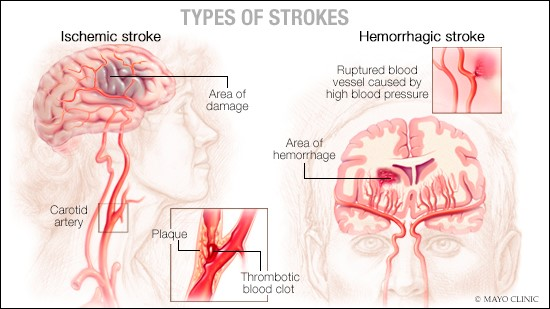
\includegraphics[width=1.1\linewidth]{figures/ch2/strokecauses}
	\caption{Figure showing the causes and Main types of stroke \cite{mayostroke}.}
	\label{fig:brain}
\end{figure}

\begin{figure}[p]%figure effects
	\centering
	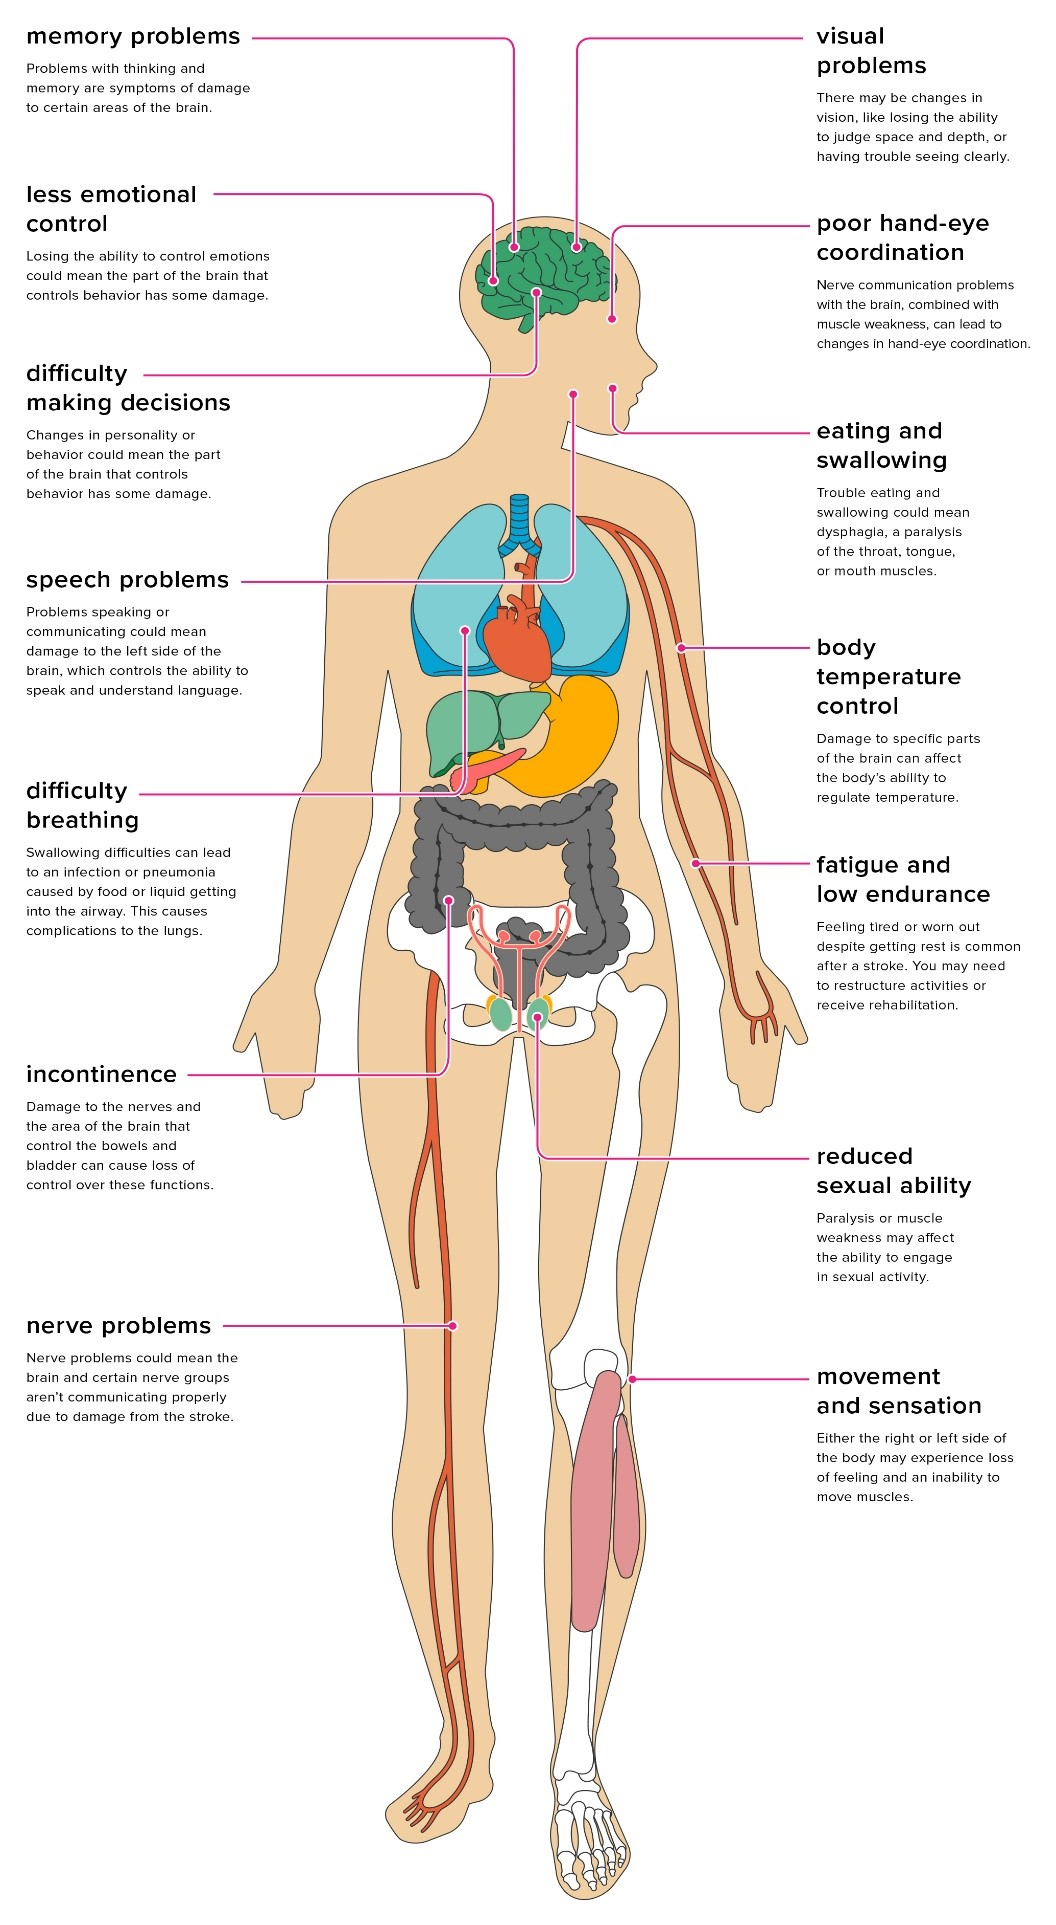
\includegraphics[height=22cm]{figures/ch2/strokeeffects}
	\caption{Figure showing the effects on the body from Stroke \cite{Marcin2019}.}
	\label{fig:effects}
\end{figure}
\newpage

\subsection{Stroke Symptoms}
Since Stroke is a medical emergency, early recognition of its symptoms can help in prompt treatment for such patients, \cite{mayosym} the signs that a person is experiencing a stroke include:
\begin{itemize}%symptoms list
	\item \textbf{Trouble speaking and understanding what others are saying.} 	 There might be an experience of confusion, slurring of words or having a difficulty understanding speech.
	\item \textbf{Paralysis or numbness of the face, arm and leg.} There might be a development of sudden numbness, weakness or paralysis in the face, arm or leg, this often affects only one side of the body. A way to test for this is for the person to raise both their arms above their head and if one arm begins to fall it means the person in question might have a stroke.
	\item \textbf{Problems seeing in one or both eyes.} Sudden blurred or blackened vision in one or both eyes, and seeing double
	\item \textbf{Headache.} A sudden headache accompanied by vomiting, dizziness or altered consciousness may indicate stroke
	\item \textbf{Trouble walking.}  When walking and you stumble or lose one’s balance, there may also be sudden dizziness or loss of coordination.
\end{itemize}

If any of the signs have been noticed there is also a check for being sure of the symptoms and it is known as “FAST”\\
\begin{itemize}%fast list
	\item[\textbf{F:}]\textbf{ Face.} Ask the person to smile, does one side of the face droop?
	\item[\textbf{A:}]\textbf{ Arms.} Ask the person to raise both arms. Does one arm drift downward? Or is one arm usable to rise.
	\item[\textbf{S:}]\textbf{ Speech.} Ask the person to repeat a simple phrase, is his or her speech slurred or strange.
	\item[\textbf{T:}]\textbf{ Time.} If you observe any of these signs call emergency medical help immediately.
\end{itemize}


\subsection{Stroke Risk Factors }
There are many factors that can increases a person’s stroke risk, they can be divided into lifestyle risk factors, medical risk factors and other factors \cite{mayostroke}.\\
Lifestyle risk factors are factors external to the body that a person indulges in that can increase their stroke risk, While Medical risk factors are those which originate from the body, can be innate or through sickness. examples of lifestyle and medical risk factors are:
\begin{itemize}%lifestyle & medical risk factorss
	\item[] Physical inactivity
	\item[] Heavy drinking or binge drinking
	\item[] Use of illegal drugs
	\item[] Cardiovascular disease
	\item[] Family history of stroke, heart attack or transient ischemic attack 
\end{itemize}



\subsection{Stroke Complications}
A stroke can sometimes cause temporary or permanent disabilities depending on how long the brain lacks blood flow and which part was affected. Complications may include the following and they are also indicated in Figure \ref{fig:effects}:
\begin{itemize}%complications list
	\item Paralysis or loss of muscle movement. a person may be paralyzed if the part of the brain responsible for the movement of that limb is affected.
	\item Difficulty talking or swallowing. A stroke may affect control of the muscles in the mouth and throat resulting in difficulty talking, swallowing and eating. There can also be difficulty with language including speaking or understanding speech, reading or writing.
	\item Memory loss or thinking difficulties. Many people who have had stroke experience some memory loss. Others may have difficulty thinking, reasoning, making judgements and understanding concepts.
	\item Emotional problems. People who have had stroke may have more difficulty controlling their emotions, or they may develop depression.
	\item Pain. Pain, numbness or other unusual sensations may occur in the parts of the body affected by stroke.
	\item Changes in behavior and self-care ability. People who have had stroke may become more withdrawn. They may need help with grooming and daily chores.
\end{itemize}

\subsection{Stroke Recovery and Rehabilitation}
After emergency treatment patients are usually monitored for at least a day, after which stroke care in then focused on helping the patient recover as much function as possible so the patient can return to independent living. The impact on the brain from stroke depends on the area of the brain involved and the amount of tissue damaged, if the stroke affected the right side of the brain, movement and sensation on the left side may be affected and same for the left side of the brain and the right side of the body. And brain damage to the left side of the brain can cause speech and language disorders. \\
The Stroke rehabilitation process can be described as a cycle that involves: assessment of the patient’s needs, goal setting for improvement, intervention to assist with said goals, and reassessment at some periodic time to assess the progress towards the goal. \cite{mayostroke,eggers1984occupational}\\
The future effect of stroke on a patient is dependent on the site and size of the initial stroke lesion and the extent of the recovery. Recovery is through a combination of learning-dependent processing that included restitution, substitution, and compensation. Even though stroke recovery is unique the recovery in the first days are predictable \cite{Langhorne2011a}. Therefore, it is important to start the recovery process to allow for large gains in functional ability, shown in Figure\ref{fig:recovery}.

\begin{figure}[p]%figure of recovery curve
	\centering
	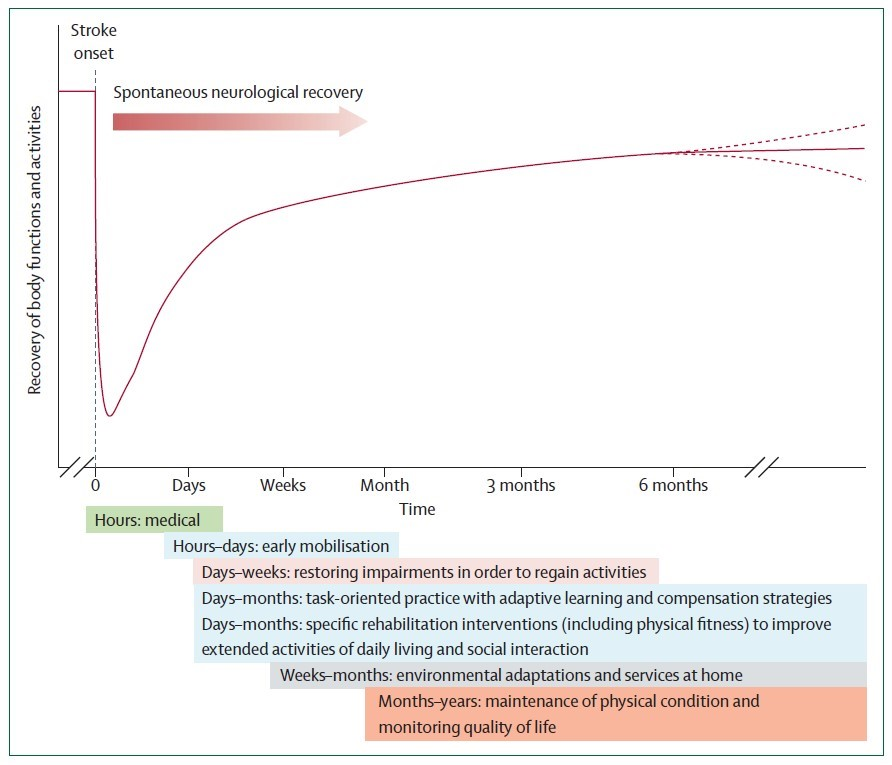
\includegraphics[width=14cm,height=10cm]{figures/ch2/recpattern}
	\caption{A figure showing the hypothetical pattern of recovery after stroke with timing of intervention strategies \cite{Langhorne2011a}.}
	\label{fig:recovery}
\end{figure}
\newpage
\section{Rehabilitation Robots}\label{sec:rehabrobots}
\subsection{What is Rehabilitation}
Rehabilitation can be defined as \begin{quotation}
	\textit{``a set of interventions designed to optimize functioning and reduce disability in individuals with health conditions in interaction with their environment''}\\
	\begin{flushright}
		\cite{Sjolund2013}
	\end{flushright}
\end{quotation}.
Rehabilitation as described by Eggers \cite{eggers1984occupational}, says that the end goal of rehabilitation should not only be the conscious use of the paralysed hand. But the end goal should be to allow the paralysed hand to be able to person some of the tasks it used to do before paralysis\cite{Johnson2005}.\\
As listed in \cite{whorehab} some examples of rehabilitation include : 
\begin{itemize}%examples of rehabilitation
	\item Exercises to improve a person’s speech, language and communication after a brain injury.
	\item Modifying an older person’s home environment to improve their safety and independence at home and to reduce their risk of falls.
	\item Exercise training and education on healthy living for a person with a heart disease.
	\item Making, fitting and educating an individual to use a prosthesis after a leg amputation.
	\item Positioning and splinting techniques to assist with skin healing, reduce swelling, and to regain movement after burn surgery.
	\item Prescribing medicine to reduce muscle stiffness for a child with cerebral palsy.
	\item Psychological support for a person with depression.
	\item Training in the use of a white cane, for a person with vision loss.
\end{itemize}

\subsection{Stroke Rehabilitation}
From literature it has been found out that most of the upper limb rehabilitation therapies done are only 50\% efficient \cite{Johnson2003}, however it has also been shown in other studies that the recovery process can be improved through forced use and enhanced therapy \cite{Duncan1997}.\\
What both forced use and enhanced therapy have in common is active participation, increased practise time, increased involvement and more repetitive training \cite{Johnson2003}.This means after a stroke, a patient will typically lose a lot of their functional ability, and the best time for gaining back that ability is within the first 6 months before the stroke is considered chronic. And with task-specific training, or other methods like high-intensity training, repetitive task training and through the use of robotics to assist in the rehabilitation \cite{Dobkin2004,Langhorne2011}.\\
Rehabilitation is highly patient specific, implying that each patient with a particular form of disability must have a rehabilitation intervention and approach designed for their goals and preferences and on the magnitude of the disability.

\subsection{Rehabilitation Robots}
The process of rehabilitation involves 4 steps as listed in \cite{Laut2016}, which are to access the type and extent of impairment, set goals to direct treatment and plan intervention to meet the goals, implementing the intervention,and reassessing the impairment level after intervention, and this steps are repeated till a impairment level is reached that is acceptable by the patient.\\
Rehabilitation robots can be used to enhance any of the steps listed above. Based on Intervention the robot can be designed to intervene in a specific region of the body, Upper limbs or lower Limbs \cite{Laut2016}.Rehabilitation robots can be divided into those that help to train (robot-aided therapy), support (exoskeleton) and replace (prosthesis) impaired activities or body functions and structures. \\
Due to the shortage of therapists to perform rehabilitation there is a need for intervention in the form telerehabilitation or advanced rehabilitation robots, which are expected to assist patients to complete therapy as accurate as well as conventional methods \cite{Sheng2016}.

\subsection{Classification of Rehabilitation Robots}
There are various ways to categorize the types of rehabilitation robots, the most classification types are from \cite{Sheng2016} and a literature review carried out personally with some of the results shown in tables: \ref{tab:reviewbilateral} and \ref{tab:reviewclincal}.\\
Based on the impairment location target for intervention, rehabilitation robots can be categorized as:
\begin{itemize}%rehab robots location aim
	\item \textbf{Lower extremity rehabilitation robots}: these are rehabilitation robots for the lower extremity of the body e.g., the legs, robots for gait.
	\item \textbf{Upper extremity rehabilitation robots}: these are rehabilitation robots for the upper extremity of the body, such robot types are: hand orthosis, upper arm rehab robots, full arm exoskeletons. 
\end{itemize}
The robot in this study is a Upper extremity rehabilitation robot, this category of robots can further be classified into 3 based on the impairment location in the upper arm \cite{Sheng2016}, these classifications are: 
\begin{itemize}%upper limb classification
	\item \textbf{Hand rehabilitation robots}: these are robots that are designed to help patients recover hand movement functions such as: grasping and grabbing. They usually coexist with Arm rehabilitation robots \cite{Troncossi2016}.
	\item \textbf{Arm Rehabilitation robots}: these robots are designed to rehabilitate the Upper arm, and can either rehabilitate the whole arm together, like the \ac{ulexo} (shown in Figure:\ref{fig:ulexo}) \cite{Shen2019a,Simkins2016}.
	\item \textbf{In-clinic devices for Occupational and physical therapy}: these types of robots are made to help patients in their rehabilitation process at their home without the need to visit a specialist, one type of robot in this category is a telerehabilitation robot/system \cite{Song2016,Carignan2006,Laut2016,Sheng2016}.
\end{itemize}
Robots that perform their tasks effectively have means to interact with their environment to perform and complete their tasks, for rehabilitation robots they need to have a connector that allows them to move the patients limbs to allow for rehabilitation of the muscles, based on this methodology there are 2 methods of patient robot interaction for Upper limb rehabilitation robots which are:
\begin{itemize}%human interaction
	\item \textbf{End-effector systems}: these are system that have an end effector (usually a handle), that the patient holds to interact with the robot. These only control from the contact area, usually the hands and require complex algorithms to be able to accurately control the movement of arm along the required path. There are other forms of interaction though games and VR. Examples of Robots like this are the \ac{mime} and \ac{arcmime} \cite{Mahoney2003,OMalley2006}, the \ac{biadler} (shown in Figure: \ref{fig:biadler}) \cite{Lott2016,Johnson2011b}, and others.
	\item \textbf{Exoskeleton systems}: these are systems whose mechanisms  cover the body part to be rehabilitated and they control the precise movement unlike the end-effector systems but they can be dangerous on the patient if not accurately designed and tested. Examples are  \ac{ulexo} (shown in Figure \ref{fig:ulexo}) \cite{Kim2013,Simkins2016}, and the HARMONY rehabilitation robot \cite{Kim2017}.
\end{itemize}
Rehabilitation robots, like all other robots have to perform their functions within a specified region which is called their workspace, based on this definition rehabilitation robots can be classified based on the type of workspace they operate in, there are 2 types of workspace that have been used by rehabilitation robots so far \cite{Sheng2016}, these classifications are:
\begin{itemize}%rehab robot task area
	\item \textbf{Planar workspace}: This workspace describes a robot only being able to act along a line or on a square on a table. The robots that use this workspace types are simple in design, thus the reason there are more commercial planar robots available like the \ac{bmt} (shown in Figure:\ref{fig:bmt}) \cite{Hesse2006,Hsieh2016,Schmidt2004}, and the MIT-MANUS \cite{Hesse2003,Hogan1992,Waldner2009}. Which are some of the more popular robots. 
	\item \textbf{3D workspace}: This workspace describes the robot being able to move the subjects arm in any of the 3 Cartesian coordinates along the length the arm can move, this workspace is versatile as it is able to allow the robot to perform many daily tasks compared to the planar workspace. With this workspace the patient can practice eating tasks, drinking, carrying a cup and much more. Examples of robots that use this type of workspace are the \ac{arcmime} \cite{Mahoney2003},\ac{built} \cite{Sampson2012a}),\ac{ulexo} (shown in Figure:\ref{fig:ulexo}) \cite{Shen2019a,Simkins2016}.
\end{itemize}
\begin{figure}[p]%bimanu image
	\centering
	
	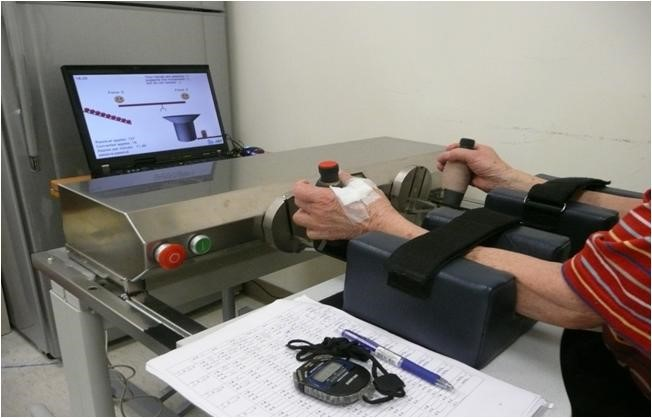
\includegraphics[width=\linewidth]{figures/ch2/bimanu}
	\caption{Picture showing a patient using the \ac{bmt}. \cite{bimanuimage}.}
	\label{fig:bmt}
\end{figure}

\begin{figure}[p]%biadler image
	\centering
	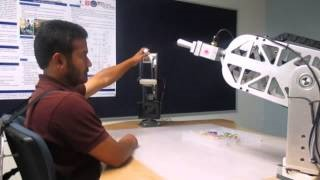
\includegraphics[width=\linewidth]{figures/ch2/biadler}
	\caption{Picture showing the \ac{biadler} being tested \cite{johnsonlab}.}
	\label{fig:biadler}
	%\label{key}
\end{figure}

\begin{figure}[p]%exoul7 image**fix position**
	\centering
	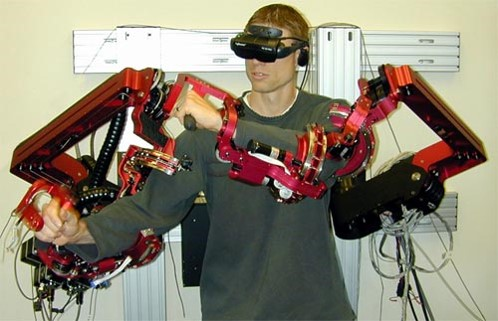
\includegraphics[width=\linewidth]{figures/ch2/ulexo}
	\caption{Figure showing a User using the \ac{ulexo} \cite{Shen2019}.}
	\label{fig:ulexo}
	%\label{key}
\end{figure}
Rehabilitation of the Upper Arm can either interact with a single arm or both arms due to the effect of the stroke, based on this definition rehabilitation robots can be classified as:
\begin{itemize}%number of arm rehabilitated
	\item \textbf{Unilateral rehabilitation}: this is the rehabilitation of only one arm/hand at a time which is usually the paretic arm \cite{Abdullah2011,Masiero2007a}.
	\item \textbf{Bilateral rehabilitation}: this is a new method that is becoming increasingly more popular with more studies showing that rehabilitating both arms together can achieve a better result faster than a unilateral therapy, and it also engages the users more,  by having them in some control modes use their more active arm to move both arms \cite{Lum1999,VanDelden2015,Wu2013,Tijs2006,Simkins2016,Shen2019a,Hsieh2016,Zhang2018,Stoykov2010}
\end{itemize}
Rehabilitation robots are built to move the impaired arm along a particular path, but in general there are some methods that are commonly used by researchers developing or using commercial robots, some of these training method/ control modes are:
\begin{itemize}\label{list:scontrol}%control modes for rehab robots
	\item \textbf{The bilateral modes of passive-passive, active-passive and active-active control modes}: this mode is seen on the \ac{mime} and \ac{arcmime} and it describes the type of activity on each arm, passive being the robot moves the arm, active being the arm has to move against a resistive force.
	\item \textbf{Master slave bilateral robot mode}: this is the control mode that is generally seen in 3D workspace rehabilitation robots, because there is no control strategy that has been seen to able to solve the problem of controlling both hands, this method makes the slave arm (connected to the paretic arm) to follow the motion of the Master arm(connected to the stronger arm) and it has been shown to work well \cite{Guo2013,Harischandra2017,Liu2010,Lott2016,Sheng2018,Shen2019a}.
	\item\textbf{ \ac{arcmime} modes of active constrained and bimanual mode}: this modes are used on both the \ac{mime} and \ac{arcmime} robots, the robots also include active and passive modes, the bimanual allows for both arms to be used for rehabilitation \cite{Mahoney2003,Waldner2009}.
	\item \textbf{Resistive and assistive rehabilitation}: this control modes describes whether the robot helps the patients to perform the task (assistive), or the robot provides a constant or varying resistive force to their action to allow them use their force (resistive). These are popular among linear planer rehabilitation robots \cite{Haghshenas-Jaryani2020,Zollo2011}.
\end{itemize}


\newpage
\subsection{Literature Review on Existing Rehabilitation robots}
Due to there being a lack of up-to-date information on Bilateral rehabilitation robots, there was a need for a literature review survey on the current state of the art in the aspect of  rehabilitation robots, that is what these reviews are aimed to solve. \\
Table \ref{tab:reviewclincal} shows details from papers from 1980 to 2020 that involved a clinical trial with a bilateral robot. Important details of note are: number of patients involved the trial. Amount of patienta within each stroke period of time, average time after stroke, intervention used, FES use involved, outcome measures used, details of intervention measures. All of which make each entry to be different from each other based on the experiment goal and patients available for testing.\\
Table \ref{tab:reviewbilateral} contains a summary of each paper reviewed and  the methods used.

\newpage
\section{Force-Torque Sensors}
\subsection{Definition of Force-Torque Sensors.}
A Force-Torque Sensor is an electronic transducers that are made up of \ac{fsr} \cite{Florez2010} that allow the transducer to be able to measure static or dynamic forces applied to its surface, through the variation of it's resistance, while a multi axis force sensor is a device that measures the outputting forces and torques from all three Cartesian coordinates (x, y, and z). A six-axis force/torque transducer is also known as a multi-axis force/torque transducer, multi-axis load cell, F/T sensor, or six-axis load cell \cite{atifts}.\\
The Importance to be able to measure all the 6 components of a generalized force is important in many testing and implementations such as force sensors for: wind tunnels, robotics, general structures \cite{Ballo2014,ATI2013,Jost2020}, with an example of commercial force sensors for general purposes shown in Figures: \ref{fig:atifs} and \ref{fig:comfs}.

\subsection{Importance of Force-Torque sensors in Rehabilitation robots.}
The need for force-sensors has been increasing due to the advances and increase in amount of human-robot interaction and robots that need to interact with humans \cite{Kim2017}. A robotic end-effector is any object attached to the robot flange (wrist) that serves a function. This includes robotic grippers, robotic tool changers, robotic collision sensors, robotic rotary joints, robotic press tooling, compliance devices, robotic paint guns, material removal tools, robotic arc welding guns, robotic transguns, etc. Robot end-effectors are also known as robotic peripherals, robotic accessories, robot tools, or robotic tools, \ac{eoa}, or end-of-arm devices \cite{atiende}.
Force-torque sensors are able to allow robots to be able to perform more functions, because of the availability of more data. This also applies to rehabilitation robots, force-torque sensors allow for the force being applied to the patient to be accurate and also allows for the force the patient applies during a active session to be recorded and used for data analysis.\\
Because the robot has to interact with a patient with usually high spasticity, there is a need to know how much the patient is actually putting into the rehabilitation process. A solution to this is to allow the patient to do most of the work and then allow the robot to only give minimal support through a resistive means \cite{Hesse2003}.\\
From the literature review (Tables:\ref{tab:reviewbilateral},\ref{tab:reviewclincal}) most authors made use of force sensors to serve 2 purposes: To measure the muscle strength of the patient, and to measure the amount of force the have they put into the rehabilitation process. And it also helps to monitor the force levels applied to the patients, so they don’t become dangerous \cite{Adamovich2009,Diez2018}.
\begin{figure}[p]%ati loadcell image
	\centering
	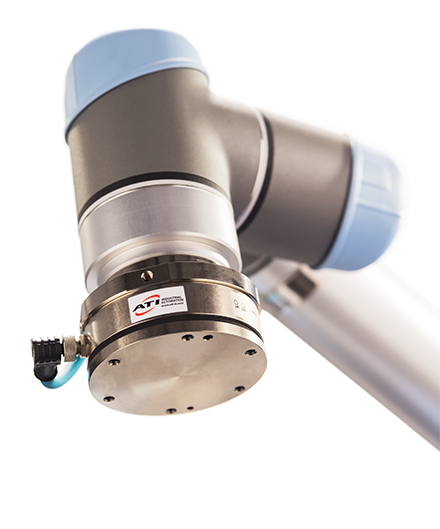
\includegraphics[height=0.5\textheight]{figures/ch2/ati}
	\caption{Figure showing an ATI force-sensor attached to the end of a \ac{ur}5 robot system \cite{atipiclink}.}
	\label{fig:atifs}
\end{figure}

\begin{figure}[p]%commercial load cell image
	\centering
	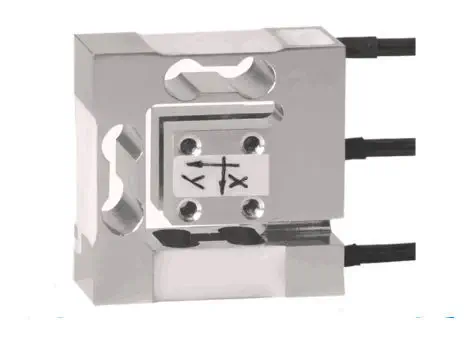
\includegraphics[width=12cm]{figures/ch2/commercialloadcell}
	\caption{Figure showing a Commercial 3-axis Force Sensor.}
	\label{fig:comfs}
\end{figure}

\newpage
\section{Transfer Learning}
\subsection{What is Transfer Learning?}
Transfer Learning or knowledge transfer are algorithm methods that are used to reduce the need and effort to recollect training data to solve multiple problems between different task domains \cite{Pan2010}.\\
From \cite{Pan2010} Transfer Learning is defined in definition \ref{def:tf}
\begin{dft}{\textbf{Transfer Learning.}}\label{def:tf}
	Given a source domain $\mathcal{D}_{\mathcal{S}}$ and a learning task $\mathcal{T}_{\mathcal{S}}$,a Target Domain $\mathcal{D}_{\mathcal{T}}$ and learning task $\mathcal{T}_{\mathcal{T}}$, transfer learning aims to help improve the learning of the target predictive function $f_{T}(.)$ in $\mathcal{D}_{T}$  using the knowledge in $\mathcal{D}_{\mathcal{S}}$ and $\mathcal{T}_{\mathcal{S}}$, where $\mathcal{D}_{\mathcal{S}}~ \neq~ \mathcal{D}_{\mathcal{T}}$ or  $\mathcal{T}_{\mathcal{S}}~\neq~ \mathcal{T}_{\mathcal{T}}$.
\end{dft}
This definition describes a situation whereby a particular problem is solved in a particular domain using a machine learning model, can we then take some of the knowledge obtained from the known model to reduce the training time for the new time by making use of the relationship between either, the problem domain, data domain and data relationship.

\subsection{Uses for Transfer Learning}
Many machine learning methods only work well only under a common assumption, which is that both the training and test data are drawn from the same feature space and distribution \cite{Pan2010}. This leads to models needing to be rebuilt using new data if the distribution or the feature space changes, which can be very expensive or impossible to get all the new data require. In such cases Transfer Learning between Domains would be desirable.\\

\subsection{Categories of Transfer Learning}
Based on the three main research issues of transfer learning: what to transfer?, how to transfer? and when to transfer? \cite{Pan2010}.
For when to transfer?, this is dependent on the problem to be solve and whether there is a need for transfer e.g. dealing with large data or lack of suitable data, that determines a need for transfer learning.\\ 
Transfer learning can be categorized based on each of the three research areas, the categorized will be described in the sections below:

\subsubsection{What to transfer?}
On the aspect of `What to Transfer?', this section is concerned with what part of the knowledge can be transferred across domains. Based on the definition above there are 4 cases for which we can choose a parameter from a model to transfer to another model \cite{Pan2010}, and these are:
\begin{itemize}
	\item[Instance ] This method assumes that some part of the data in the source domain can be reused in the target domain by re-weighting and importance sampling \cite{Pan2010,Xu2018,Cortes2007,Xia2013,Rohrbach2013,Zhang2010}.
	\item[Feature-representation] In this case, the idea is to learn a `good' representation for the target domain, meaning the knowledge to be transferred is encoded into the learned feature representation to improve performance \cite{Pan2010,Kandaswamy2014,Xia2013,Niu2021,Bahadori2014,Pan2008}. 
	\item[Parameter] In this scenario it is assumed both the source and target task share some parameters or distribution of the hyper-parameters of the models, the knowledge to be transferred is encoded into the shared parameters or priors, therefore by finding the shared parameters between domains it can be successfully be transferred \cite{Pan2010,Kumagai2016,Denil2013,Houlsby2019,Huang2010,Chapelle2000}.
	\item[Relational-knowledge] This method is similar to the parameter transfer method, but here  it is the data for both the source and target domain that are similar, therefore the knowledge to be transferred is the relationship between the data, statistical techniques are the most dominant in this field \cite{Pan2010,Niu2021,Yao2010,Tang2013,Rossi2018,Ramon2007}.
\end{itemize}

\subsubsection{How to Transfer?}
Based off the definition of transfer learning and the information from the section, transfer learning can be categorized into 3, inductive, transductive and unsupervised transfer learning, describing each in more detail below:
\begin{itemize}
	\item[Inductive ] in this scenario the source and target tasks will always be different, even though their domains might be similar, labelled data from the source is needed to induce a model for the target domain. Based on the amount of unlabelled data in the source domain this scenario can be further split into 2 cases: self-taught learning and multitask learning shown in Figure \ref{fig:pantl} \cite{Pan2010}.
	\item[Transductive] in this scenario compared to the one above, the tasks are the same, while the domains are not, it is assumed here that there is no labelled data in the target domain while there is plenty in the source domain. this scenario can be further split into 2 shown in Figure \ref{fig:pantl} which are Domain Adaptation and sample selection bias/covariance shift \cite{Pan2010}.
	\item[Unsupervised] this form is similar to the Inductive transfer learning, except it is used for solving unsupervised learning tasks in the target domain such as clustering, dimensionality reduction and density estimation \cite{Pan2010}.
\end{itemize}
\begin{figure}[p]
	\centering
	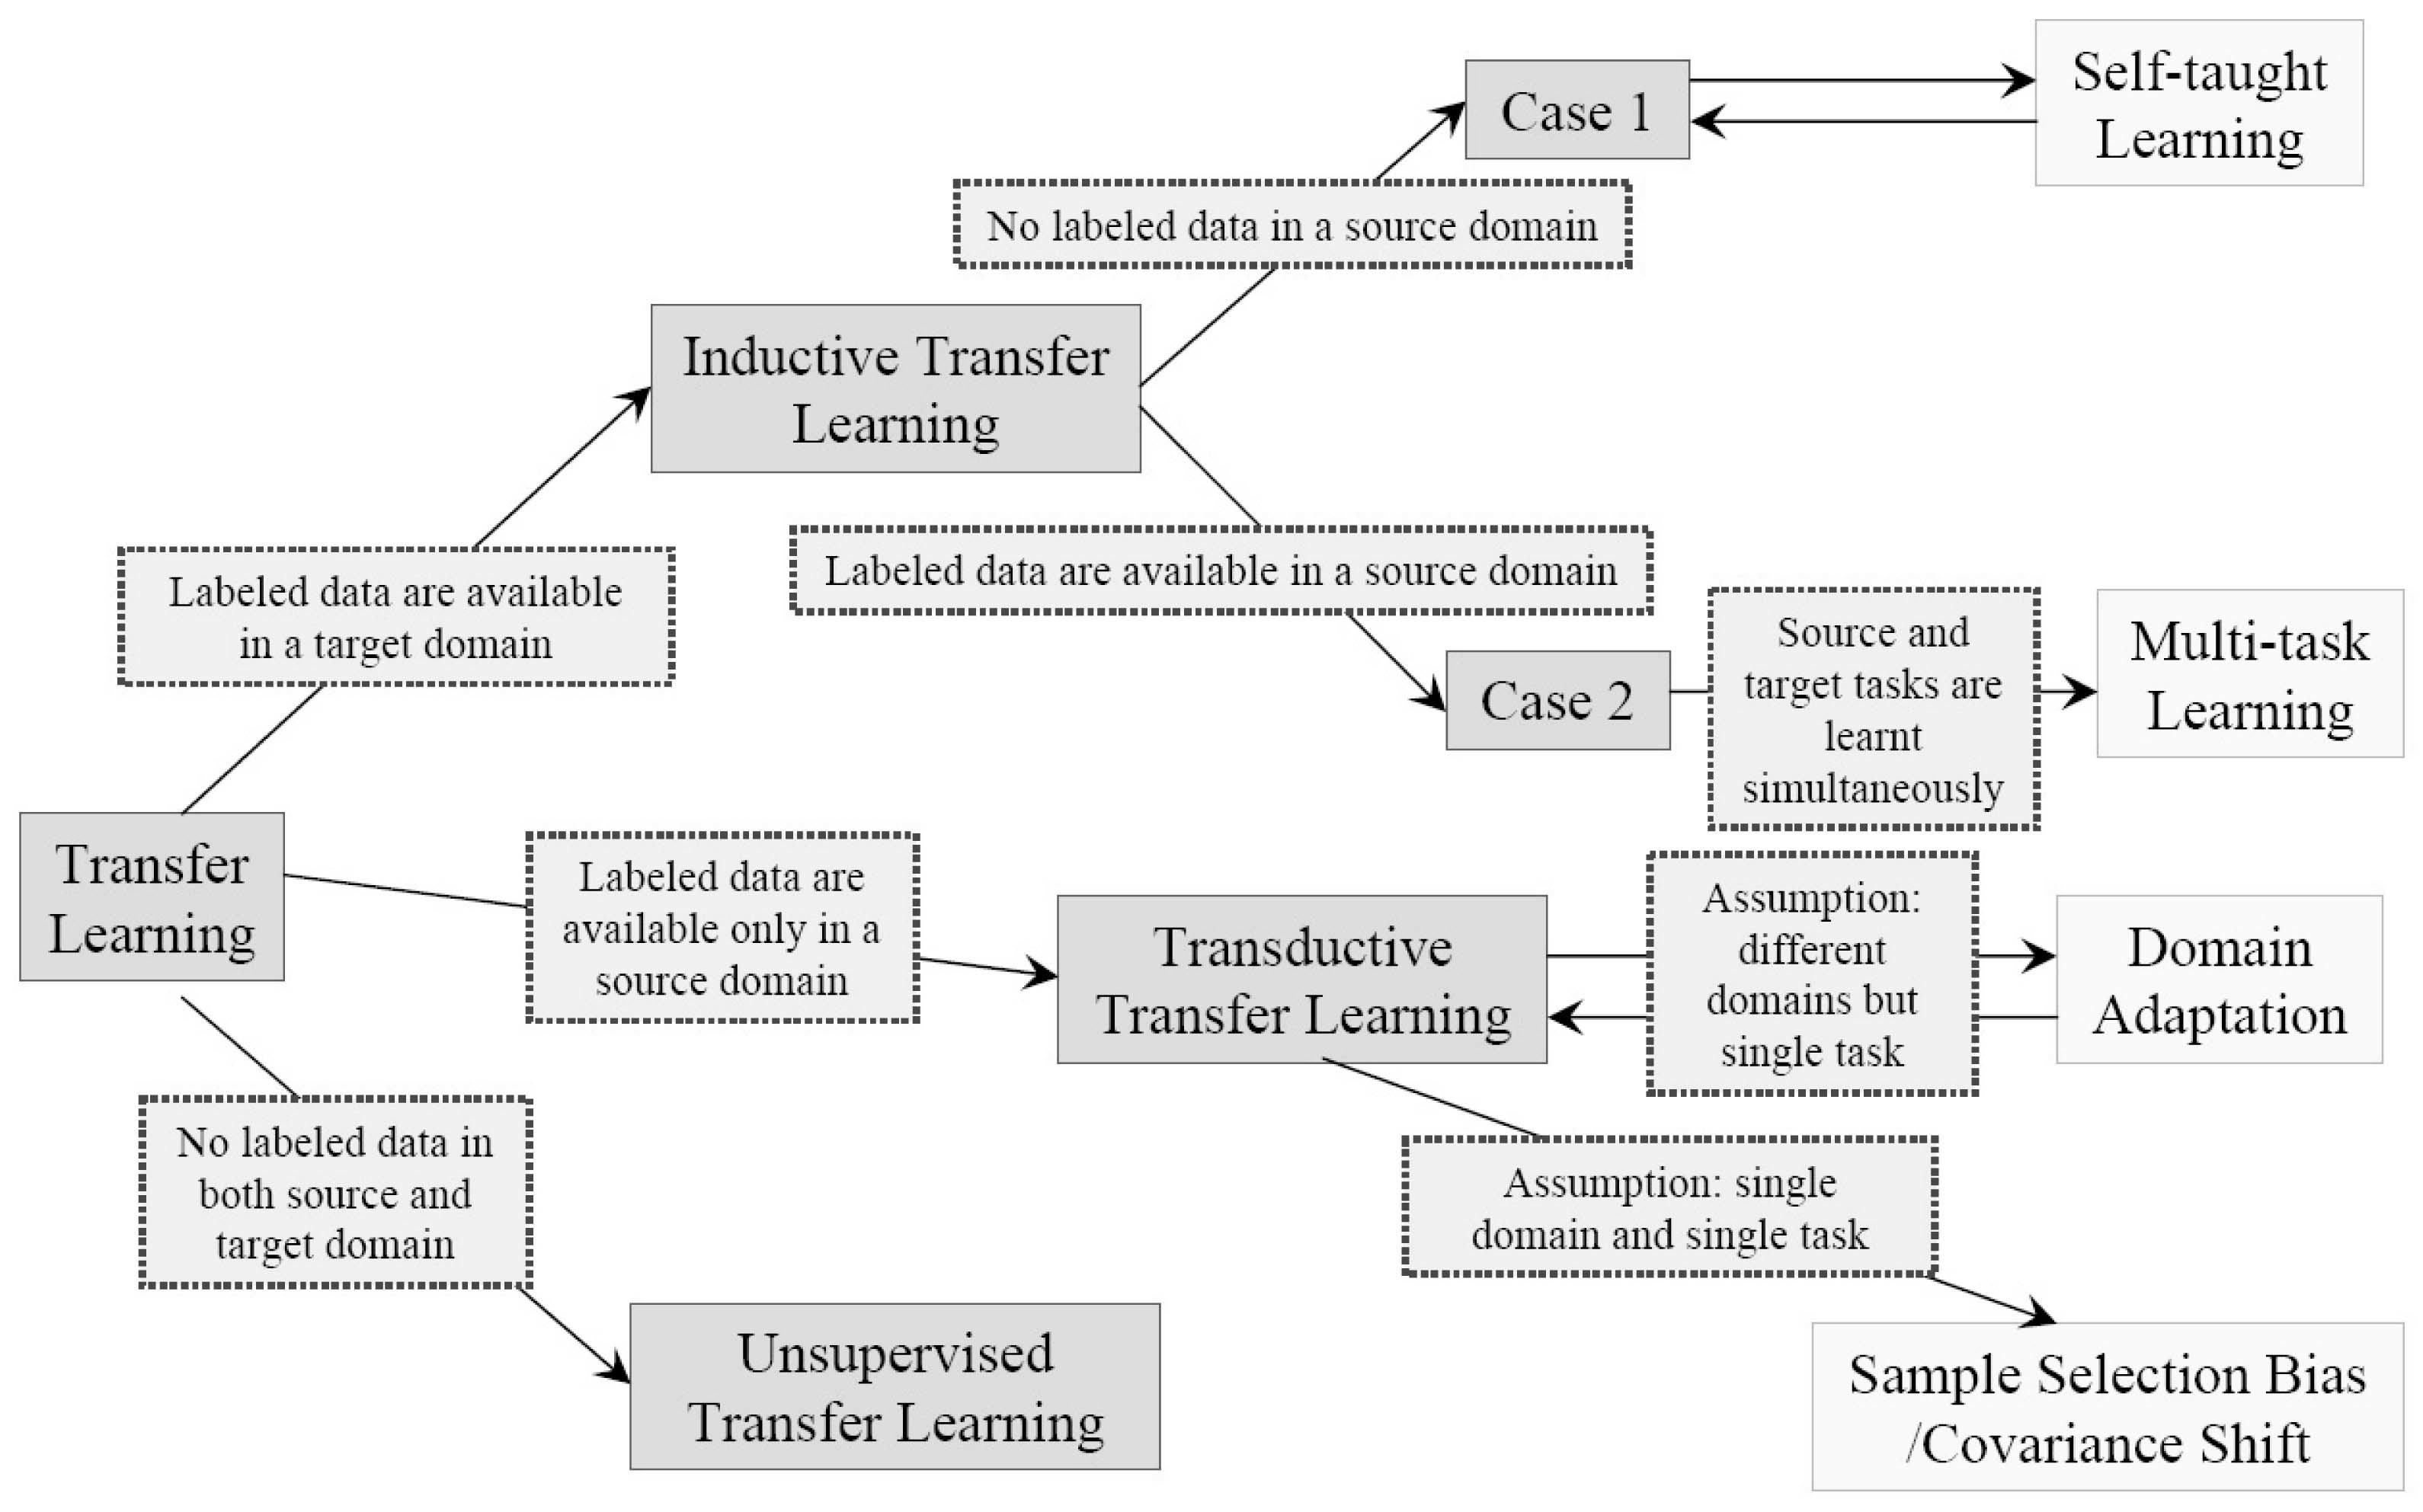
\includegraphics[width=1.1\linewidth]{figures/ch2/pantl}
	\caption{Figure showing the specification that lead to the choice of Transfer learning methods \cite{Pan2010}.}
	\label{fig:pantl}
\end{figure}
		\chapter{Methodology}\label{Ch:3}
	
\section{Design of \ac{blue}}\label{sec:Introduction3}
\subsection{Introduction to \ac{blue}}
The idea for the \ac{blue} was brought about to start designing the next rehabilitation robot that will be based on the newest technology available in rehabilitation robotics. This sprung a need for a new review on the state of robots, and in particular bilateral rehabilitation robots. This was recently done and the last proper review paper on bilateral robots was in 2016.\\
The main idea was to design a locally made version of the \acf{biadler} \cite{Christopher2014,Johnson2011a,Lott2016}, which was built to test the idea of using a robot to train specific tasks that patients lost the ability to be do because of their stroke such as: drinking, eating, reach and grabbing an object. Other researchers have done work on this topic and it led to various bilateral robots such as the \acf{ulexo} \cite{Perry2007}, the \acf{bias} system \cite{Johnson2011b}, \acf{mime} and \acf{arcmime} \cite{Burgar2011,Lum2002,Lum2005,Mahoney2003}, the \acf{bmt} \cite{Hung2019b}, the bimanual lifting rehabilitator \cite{Lum1995} and others more.

\subsection{Objectives and Specifications of \ac{blue}}
Based off the aim of the project, a list of specification can be determined for use for designing the robot. The overall desired specifications are:
\begin{itemize}%blue old specifications
	\item  3D workspace
	\item Have a suitable control method for bilateral robots
	\item similar design to the Bi-ADLER for simplicity
	\label{item:specs}
\end{itemize}
The \ac{blue} is aimed to be a Bilateral option for patient to use between it and the unilateral robot \ac{pulsr}, and to be able to quantify the difference in recovery rate between unilateral and bilateral robots.\\
%maybe remove
Due to Time Constraints, the Objectives have been simplified to 
\begin{itemize}%blue new specifications
	\item Now to be a planar bilateral robot.
	\item use a mirror-image control, as it is the suitable method for this study.
	\item Use the \ac{pulsr} arm structure as it has been analysed before.
\end{itemize}
\subsection{Design Process for \ac{blue}}
The design plan of this robot have been listed in \ref{item:specs}, and that is what is implemented in Figure \ref{fig:blue1},where the arm shown there is designed similar to the \ac{biadler} from \cite{Johnson2011}.
Simplifying the Design to suit the materials available in Nigeria, Figure \ref{fig:blue2} shows the end result of the considerations. After implementing the constraints listed above the final design for the robot is shown in Figure \ref{fig:blue3}.\\
There is also a small scare version that has been made for the purpose of demonstration of the concept shown in Figure \ref{fig:bluepres}, using parts from \ac{pulsr}2.0 and motors from \ac{pulsr}3.0 to produce the system shown in Figure \ref{fig:bluepres}.

\begin{figure}[p]%blue design 1
	\centering
	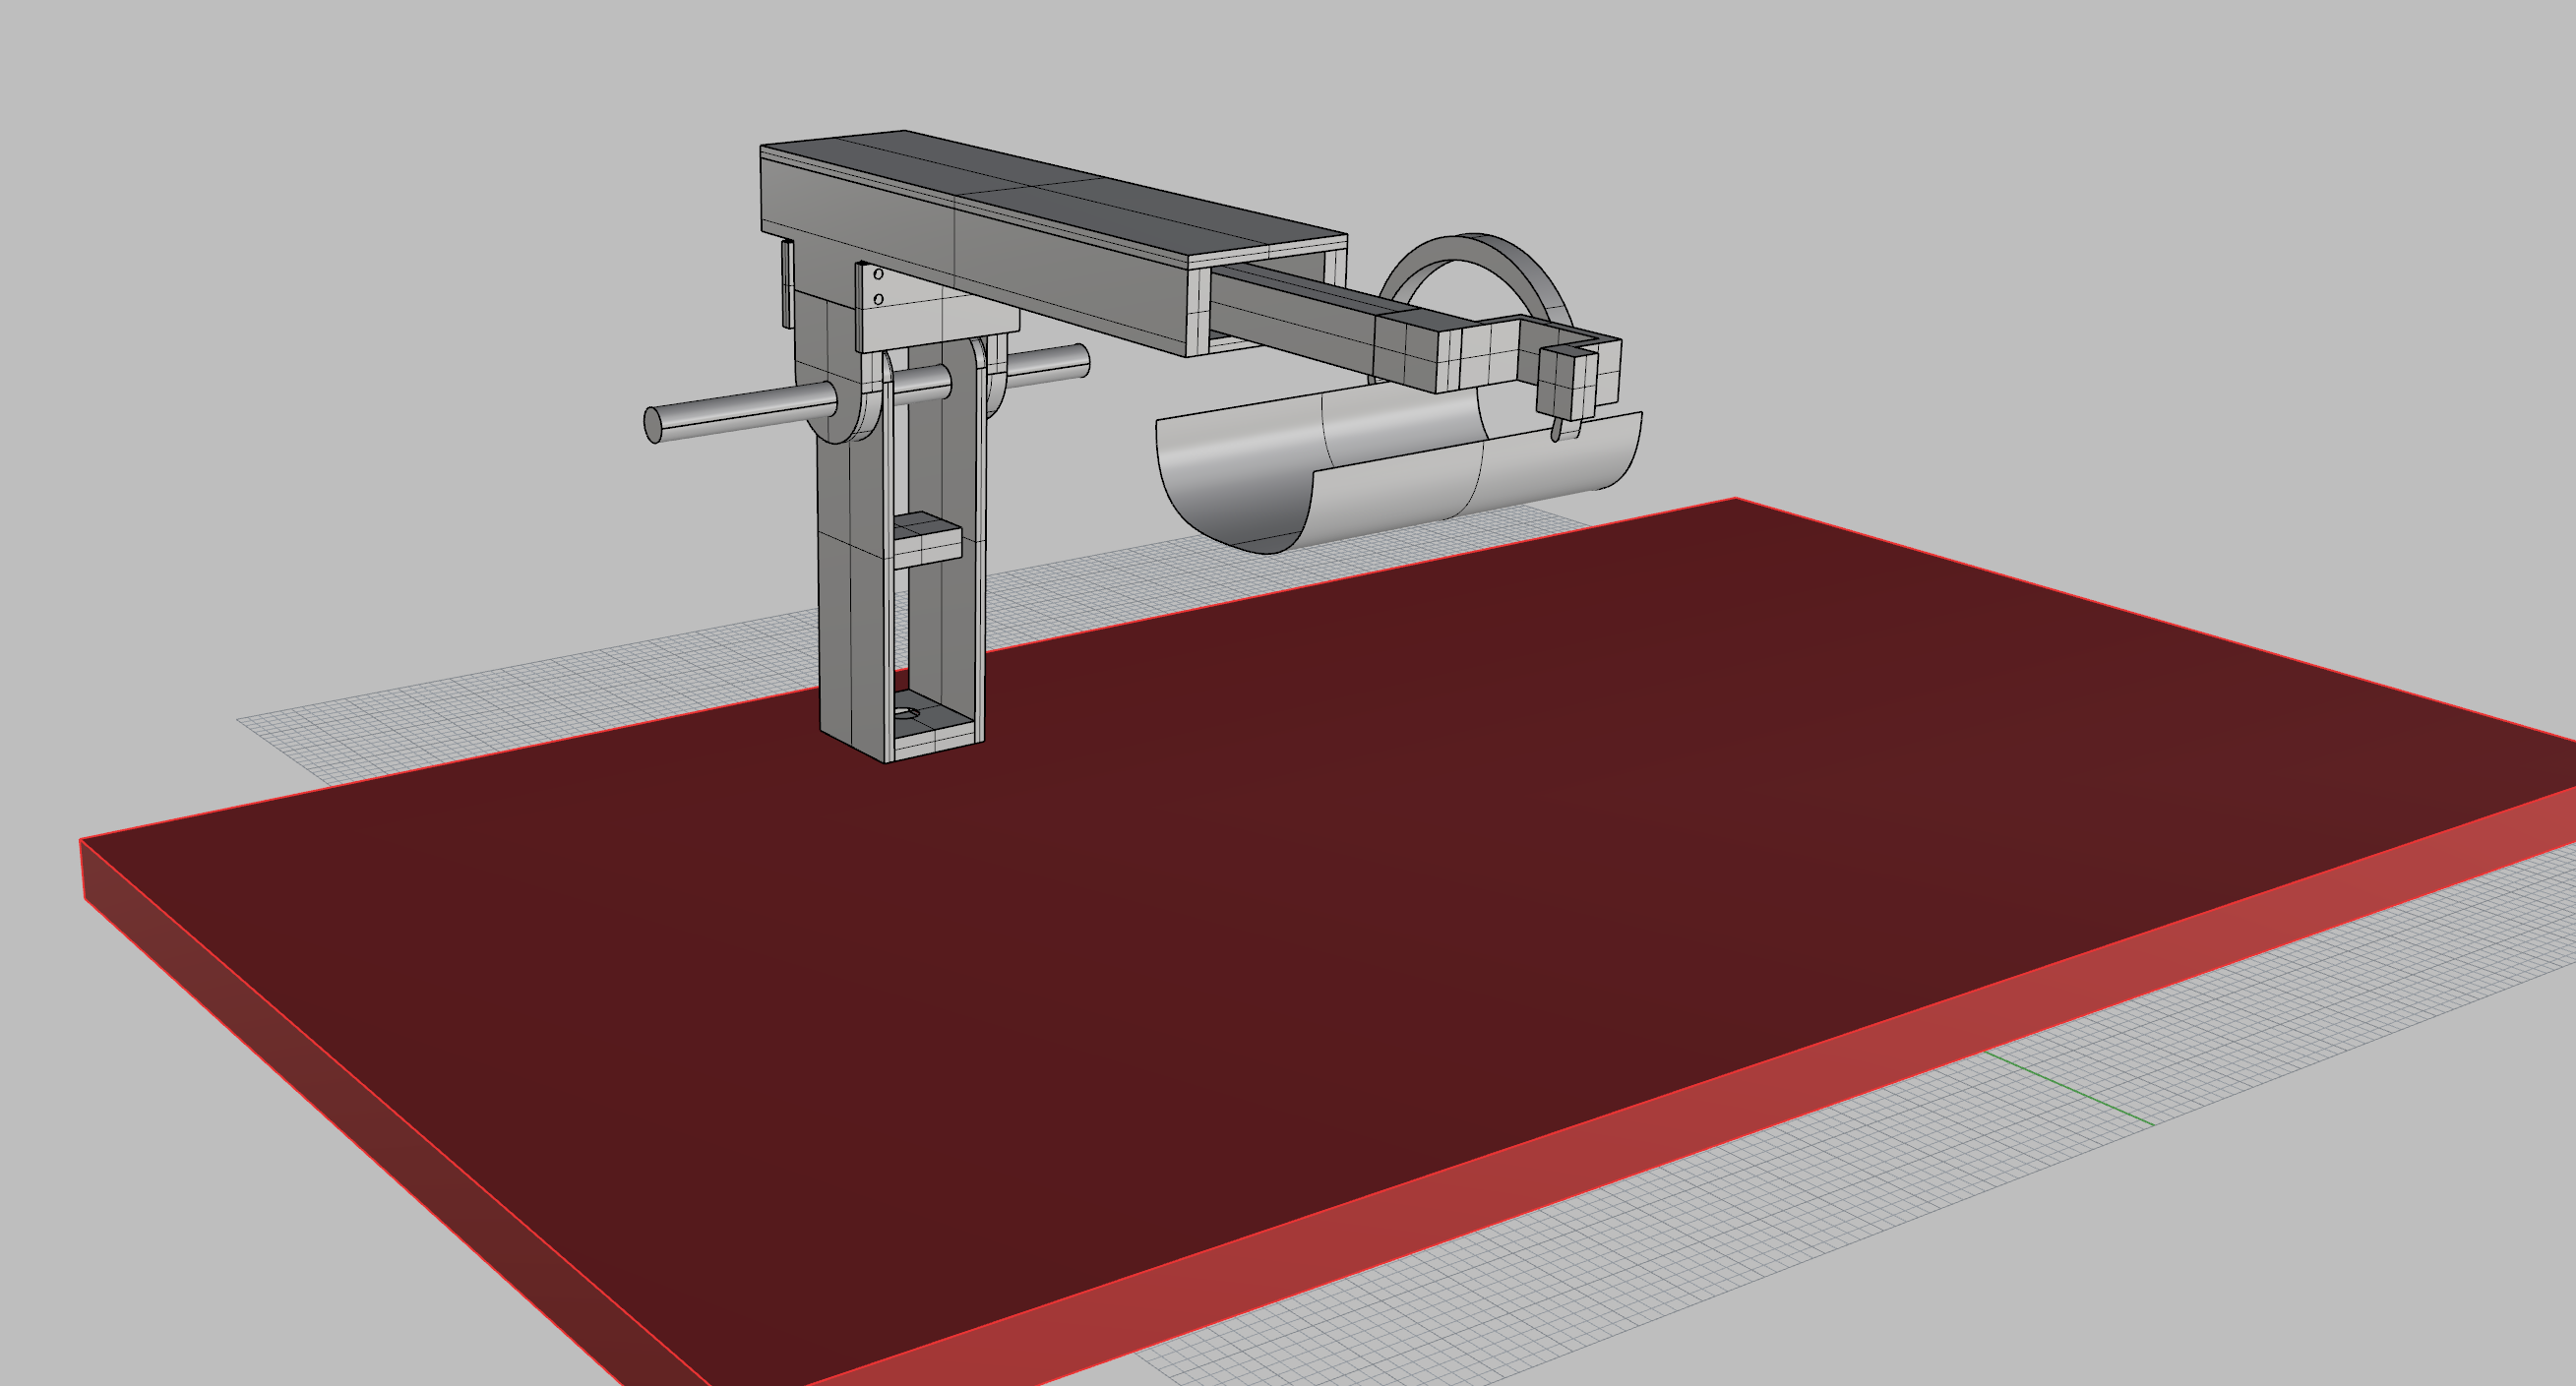
\includegraphics[width=\linewidth]{figures/ch3/bluedesign1}
	\caption{Figure showing the First proposed design of B.L.U.E.}
	\label{fig:blue1}
\end{figure}

\begin{figure}[p]%blue design 2
	\centering
	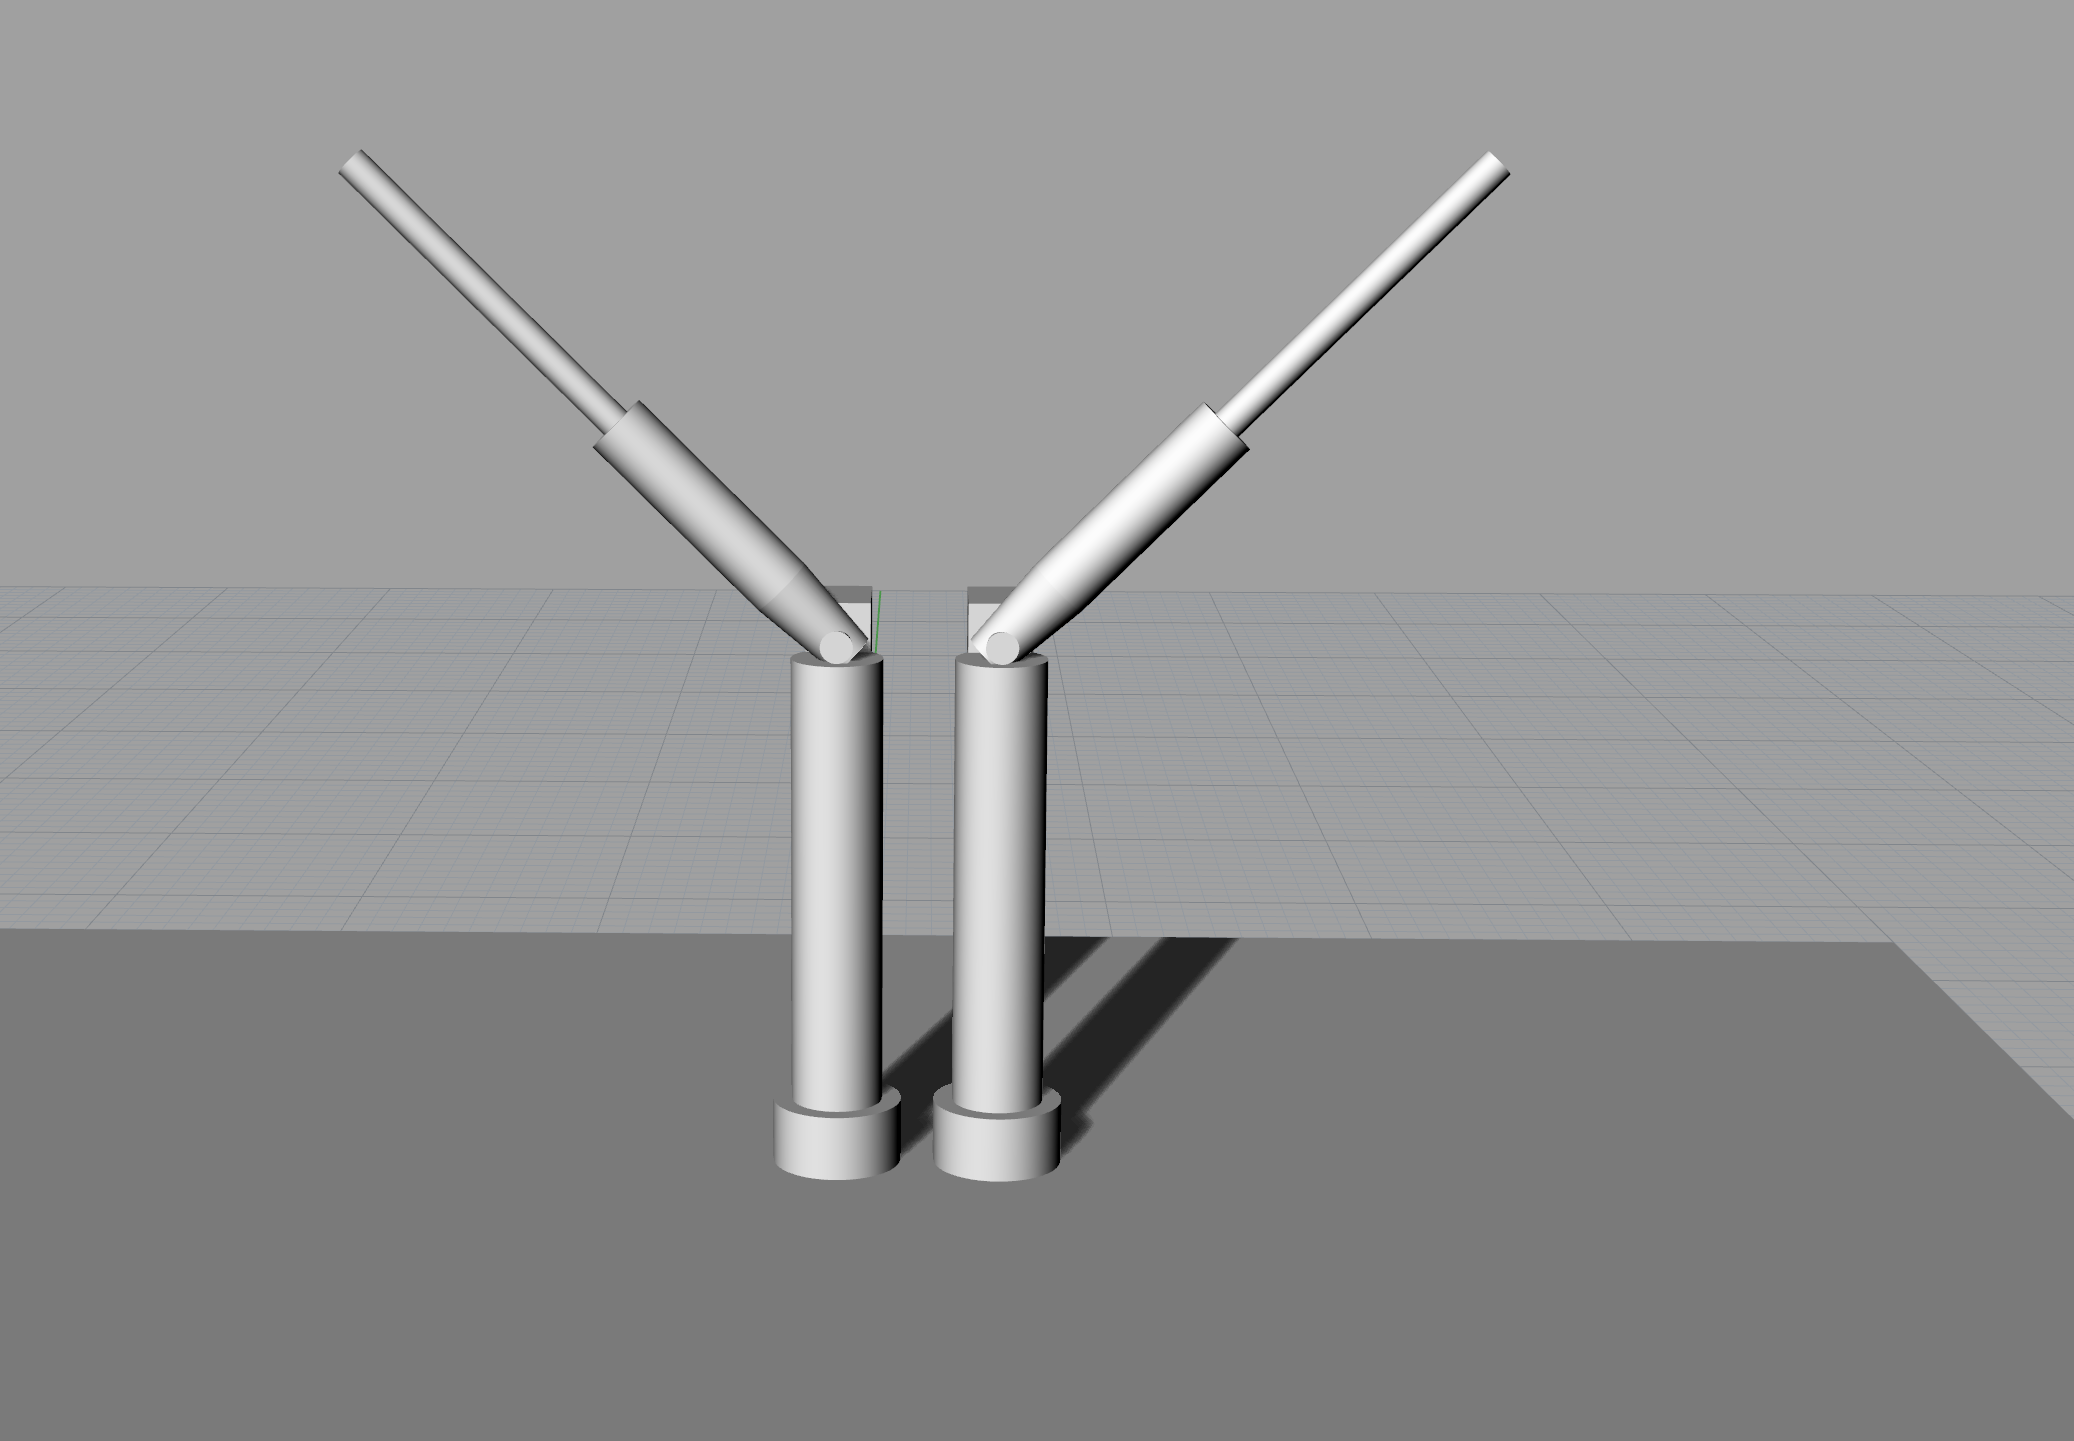
\includegraphics[width=\linewidth]{figures/ch3/bluedesign2}
	\caption{Figure showing the second proposed design of B.L.U.E.}
	\label{fig:blue2}
\end{figure}

\begin{figure}[p]%blue design 3
	\centering
	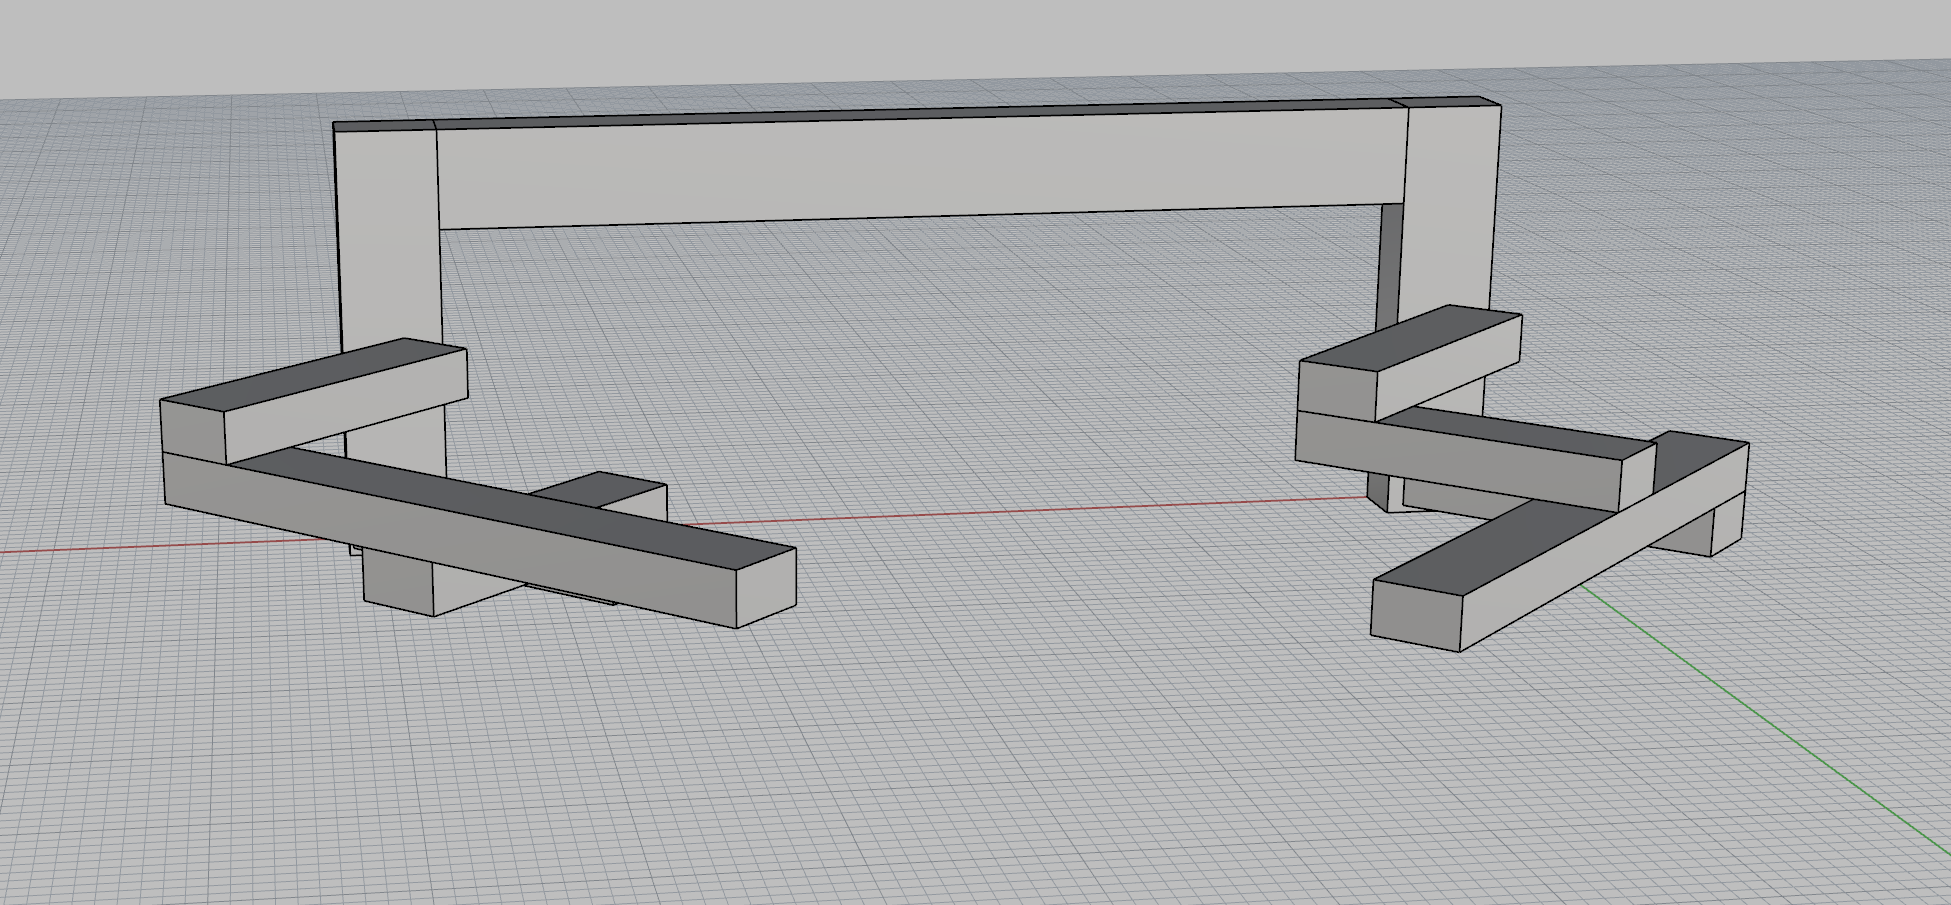
\includegraphics[width=\linewidth]{figures/ch3/bluedesign3}
	\caption{Figure showing the third proposed design of B.L.U.E.}
	\label{fig:blue3}
\end{figure}
\begin{figure}[p]%blue design presentation
	\centering
	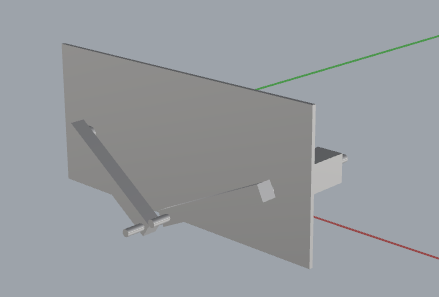
\includegraphics[width=\linewidth]{figures/ch3/bluepres}
	\caption{Figure showing the proposed Design for demonstration}
	\label{fig:bluepres}
\end{figure}
\subsection{Development of the \ac{blue} prototype}
The \ac{blue} prototype was developed as a means to show a visual representation of both a bilateral robot in action and a representation of a bilateral rehabilitation task.\\
The design used for the prototype based off the Driver's Seat robot \cite{Johnson1999,Johnson2003}, which brought about the design shown in Figure: \ref{fig:bluepres}. The materials chosen for implementation are 2 motors, 1 rotary encoder, 2 shafts with handle connectors and the control block.\\
For control of the system, a combination of both the bilateral active-passive control mode and the master-slave control mode explained in \ref{list:scontrol}, which involves a active mode on one of the motors, which will move an arm, and the master slave is implement through the rotary encoder to read the movements and tell the second motor to move in the other direction, the code to implement this is shown in the listing \ref{code:arduinomaster}.
\newpage

\section{Development of the Cascaded Force-Torque Sensor}\label{sec:forcesens}
\subsection{Design Process of the Force-Torque Sensor}
Designs on using a single-axis load cell to create a multi-axis structure had already been done in the research group before, with the result of this research producing a structure made in the design shown in Figure \ref{fig:loadcell1}.\\
Using the design above as a reference, I was able to come up with a design that measures forces in all the Cartesian axes shown in Figure \ref{fig:3dlc}. After the square brackets were made a change to the initial design was made due to the manufacturing of the load cells which meant not one of the load cells would be placed lower. The structure is design so as to behave like the commercial multi-axis force sensor shown in Figure:\ref{fig:3dlc}.\\
For the data from the load cells to be collected it is connected to a HX711 amplifier that is then connected to an arduino using the circuit connection as recommended from instructables \cite{Degraw2017} shown in Figure \ref{fig:sparkfun}, but replicated 3 times for this project.
\begin{figure}[p]%picture of assembly
	\centering
	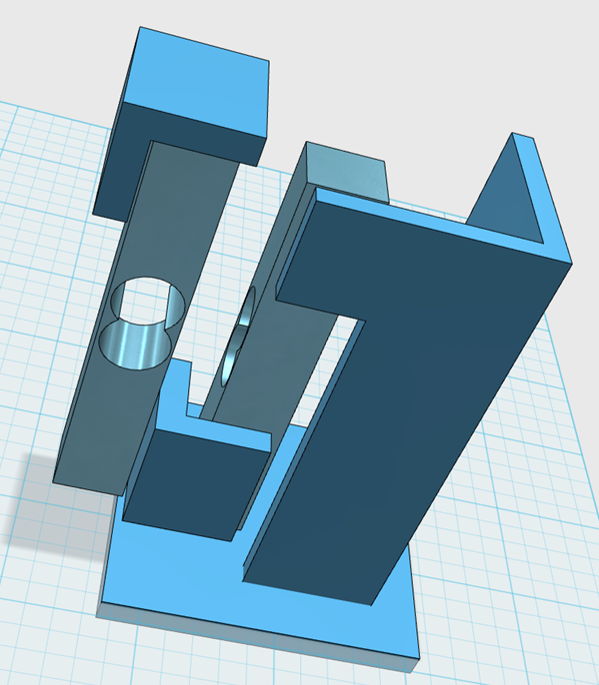
\includegraphics[width=\linewidth]{figures/ch3/loadcel1}
	\caption{Figure showing the completed assembly in testing}
	\label{fig:loadcell1}
\end{figure}

\begin{figure}[p]%forcesensorfigure
	\centering
	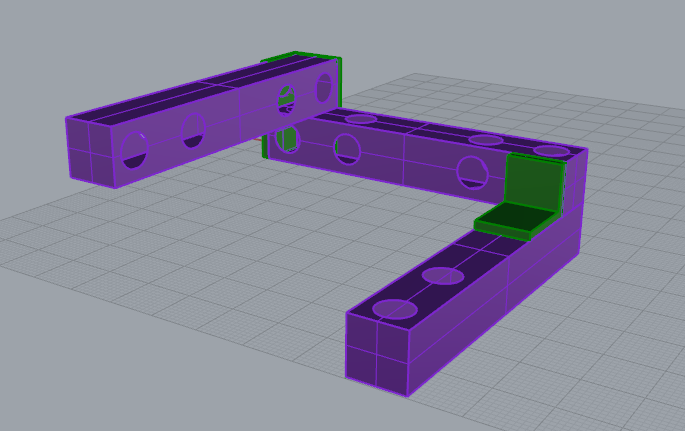
\includegraphics[width=\linewidth]{figures/ch3/loadcelldesign}
	\caption{Figure showing the first design for the 3-D force-Torque sensor}
	\label{fig:3dlc}
\end{figure}
\begin{figure}[p]%forcesensorfigure
	\centering
	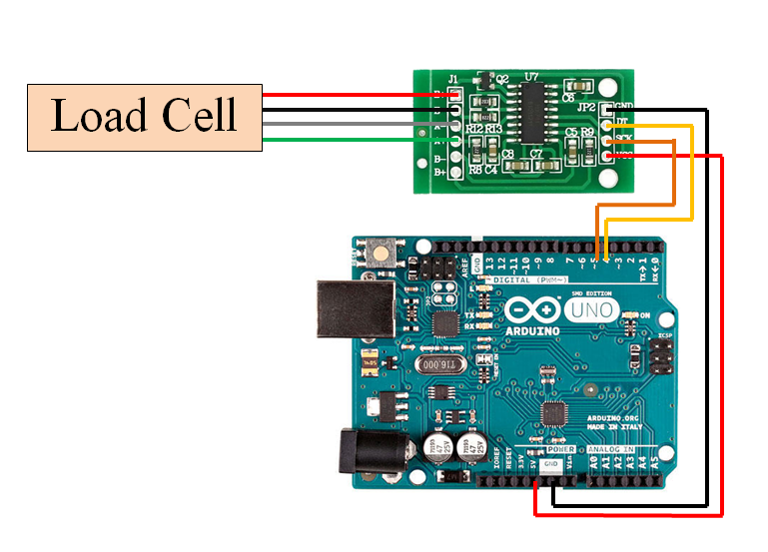
\includegraphics[width=\linewidth]{figures/ch3/sparkfun}
	\caption{Figure showing the Circuit diagram for using a commercial load cell with the HX711 amplifier \cite{Degraw2017}}
	\label{fig:sparkfun}
\end{figure}

\newpage



\subsection{Software Interface and Data Collection}
Before the load cells can be used for force measurement it has to be calibrated, the process of calibration for this system is easy and it involves having a object of known mass to then correct the calibration value till the output from the arduino matches the mass used. using the calibration code from instructables \cite{Degraw2017} shown in \ref{code:calibration} and the procedure shown in Figure \ref{fig:calibration}. Then once the calibration values have been obtained which are 5kg:361640, 10kg:220000, they can then be used in the code to obtain data for processing from the load cells.\\
After the structure had been assembled as shown in Figure \ref{fig:loadcelltest}, there was now a need for a suitable code to read from all 3 load cells simultaneously to python, for use in a transfer learning algorithm. Therefore the pyserial library was used to read data sent to the serial port from arduino that contains the data from each axis sent every 200ms, and the arduino code that sends the data to the serial shown in \ref{code:arduino}, and the python code which receives the data and saves it to a csv file is shown in \ref{code:py}.

\begin{figure}[p]%calibration images
	\centering
	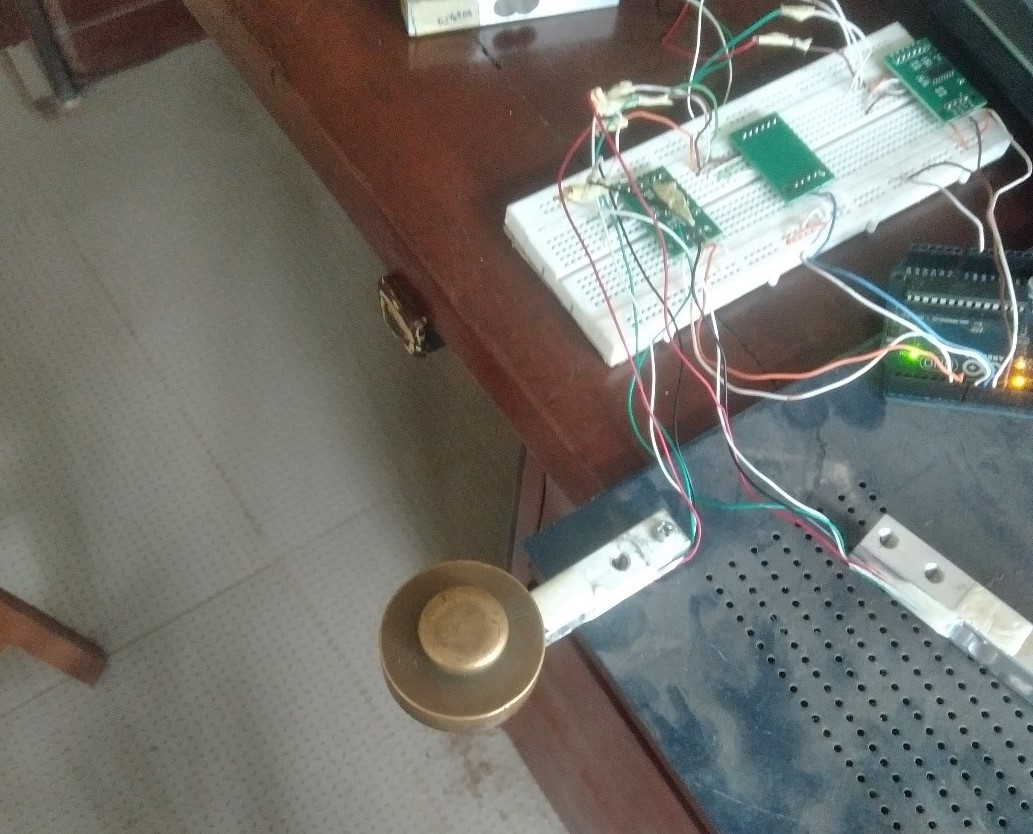
\includegraphics[width=15cm]{figures/ch3/calibration}
	\caption{Figure showing the calibration process}
	\label{fig:calibration}
\end{figure}

\begin{figure}[p]%picture of assembly
	\centering
	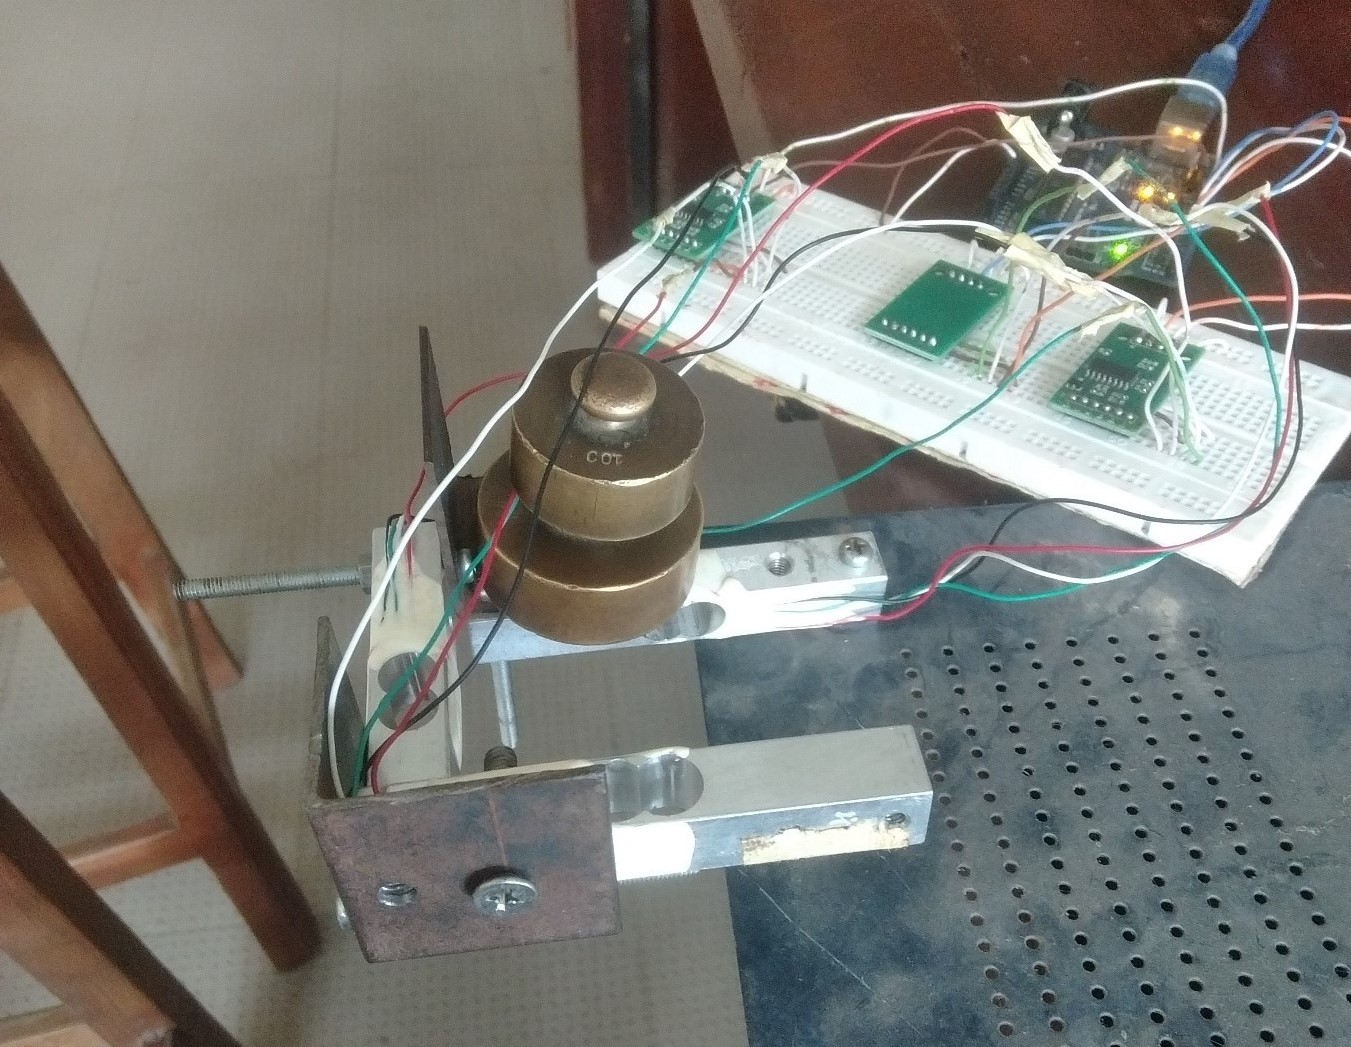
\includegraphics[width=\linewidth]{figures/ch3/loadcelltesting}
	\caption{Figure showing the completed assembly in testing}
	\label{fig:loadcelltest}
\end{figure}
\newpage
\subsection{Experiment Design and Implementation}\label{sec:experiment}
After the construction of the assembly had been completed, there is now a need to perform an experiment to confirm if the data from the novel multi-axis load cell from this study has worse prediction than a commercial multi-axis force sensor.\\
The concept of the design is to record the data from both force-sensors when the same force is applied to them both, but due to complications only data from the novel force-sensor was available for use. After the novel force sensor is assembled as it will be used, a range of force are applied to it at the end-effector point with varying magnitudes and force directions, to see the influence on the other load cells in the array, the experiment process is shown in Figure \ref{fig:loadcelltest}. The results of the test are shown in the next chapter.
%\subsection{Transfer Learning Problem Statement}

		\chapter{Results and Discussion}  \label{Ch:4}

\section{Development Results}
The methodology of construction of the novel force sensor as detailed in section \ref{sec:forcesens}, the novel force-sensor was built using the speechifications listed in the section to produce a physical version used for the comparison experiment shown in Figure: \ref{fig:loadcelltest}.\\
The novel force sensor array has been found to be able to measure the correct amount of force applied to each of the load cells in the applied direction.


\section{Results from the Experiment on force sensor}
from the experiment performed in section \ref{sec:experiment}, the force magnitude from each load cell collected from the python code \ref{code:py}, are then plotted in MATLAB, showing the significance of applying a force on the other load cells.\\
the first experiment carried out was to apply force only in the vertical axis and measure co-linearities measures across the other load cells, the results from this experiment are shown in Figure:\ref{fig:matlab1}, and from the plot we can see from 1 to 300, the forces applied is only read majorly by the y-axis load cell but after that, there is a lot of interference in the other load cells, mostly due to the unstable structure will allows the load cells to move and couple each other.\\
For the second experiment, varied force is applied in the positive and negative directions of each axis to see the effect, shown in Figure \ref{fig:matlab2}. It is seen that when negative and positive y forces are applied there is little effect on the other load cells, unlike the z-axis where negative z shows a very large deflection on the other load cells, same for the x-axis load cell as well.

\begin{figure}[p]%matlab result graph 1
	\centering
	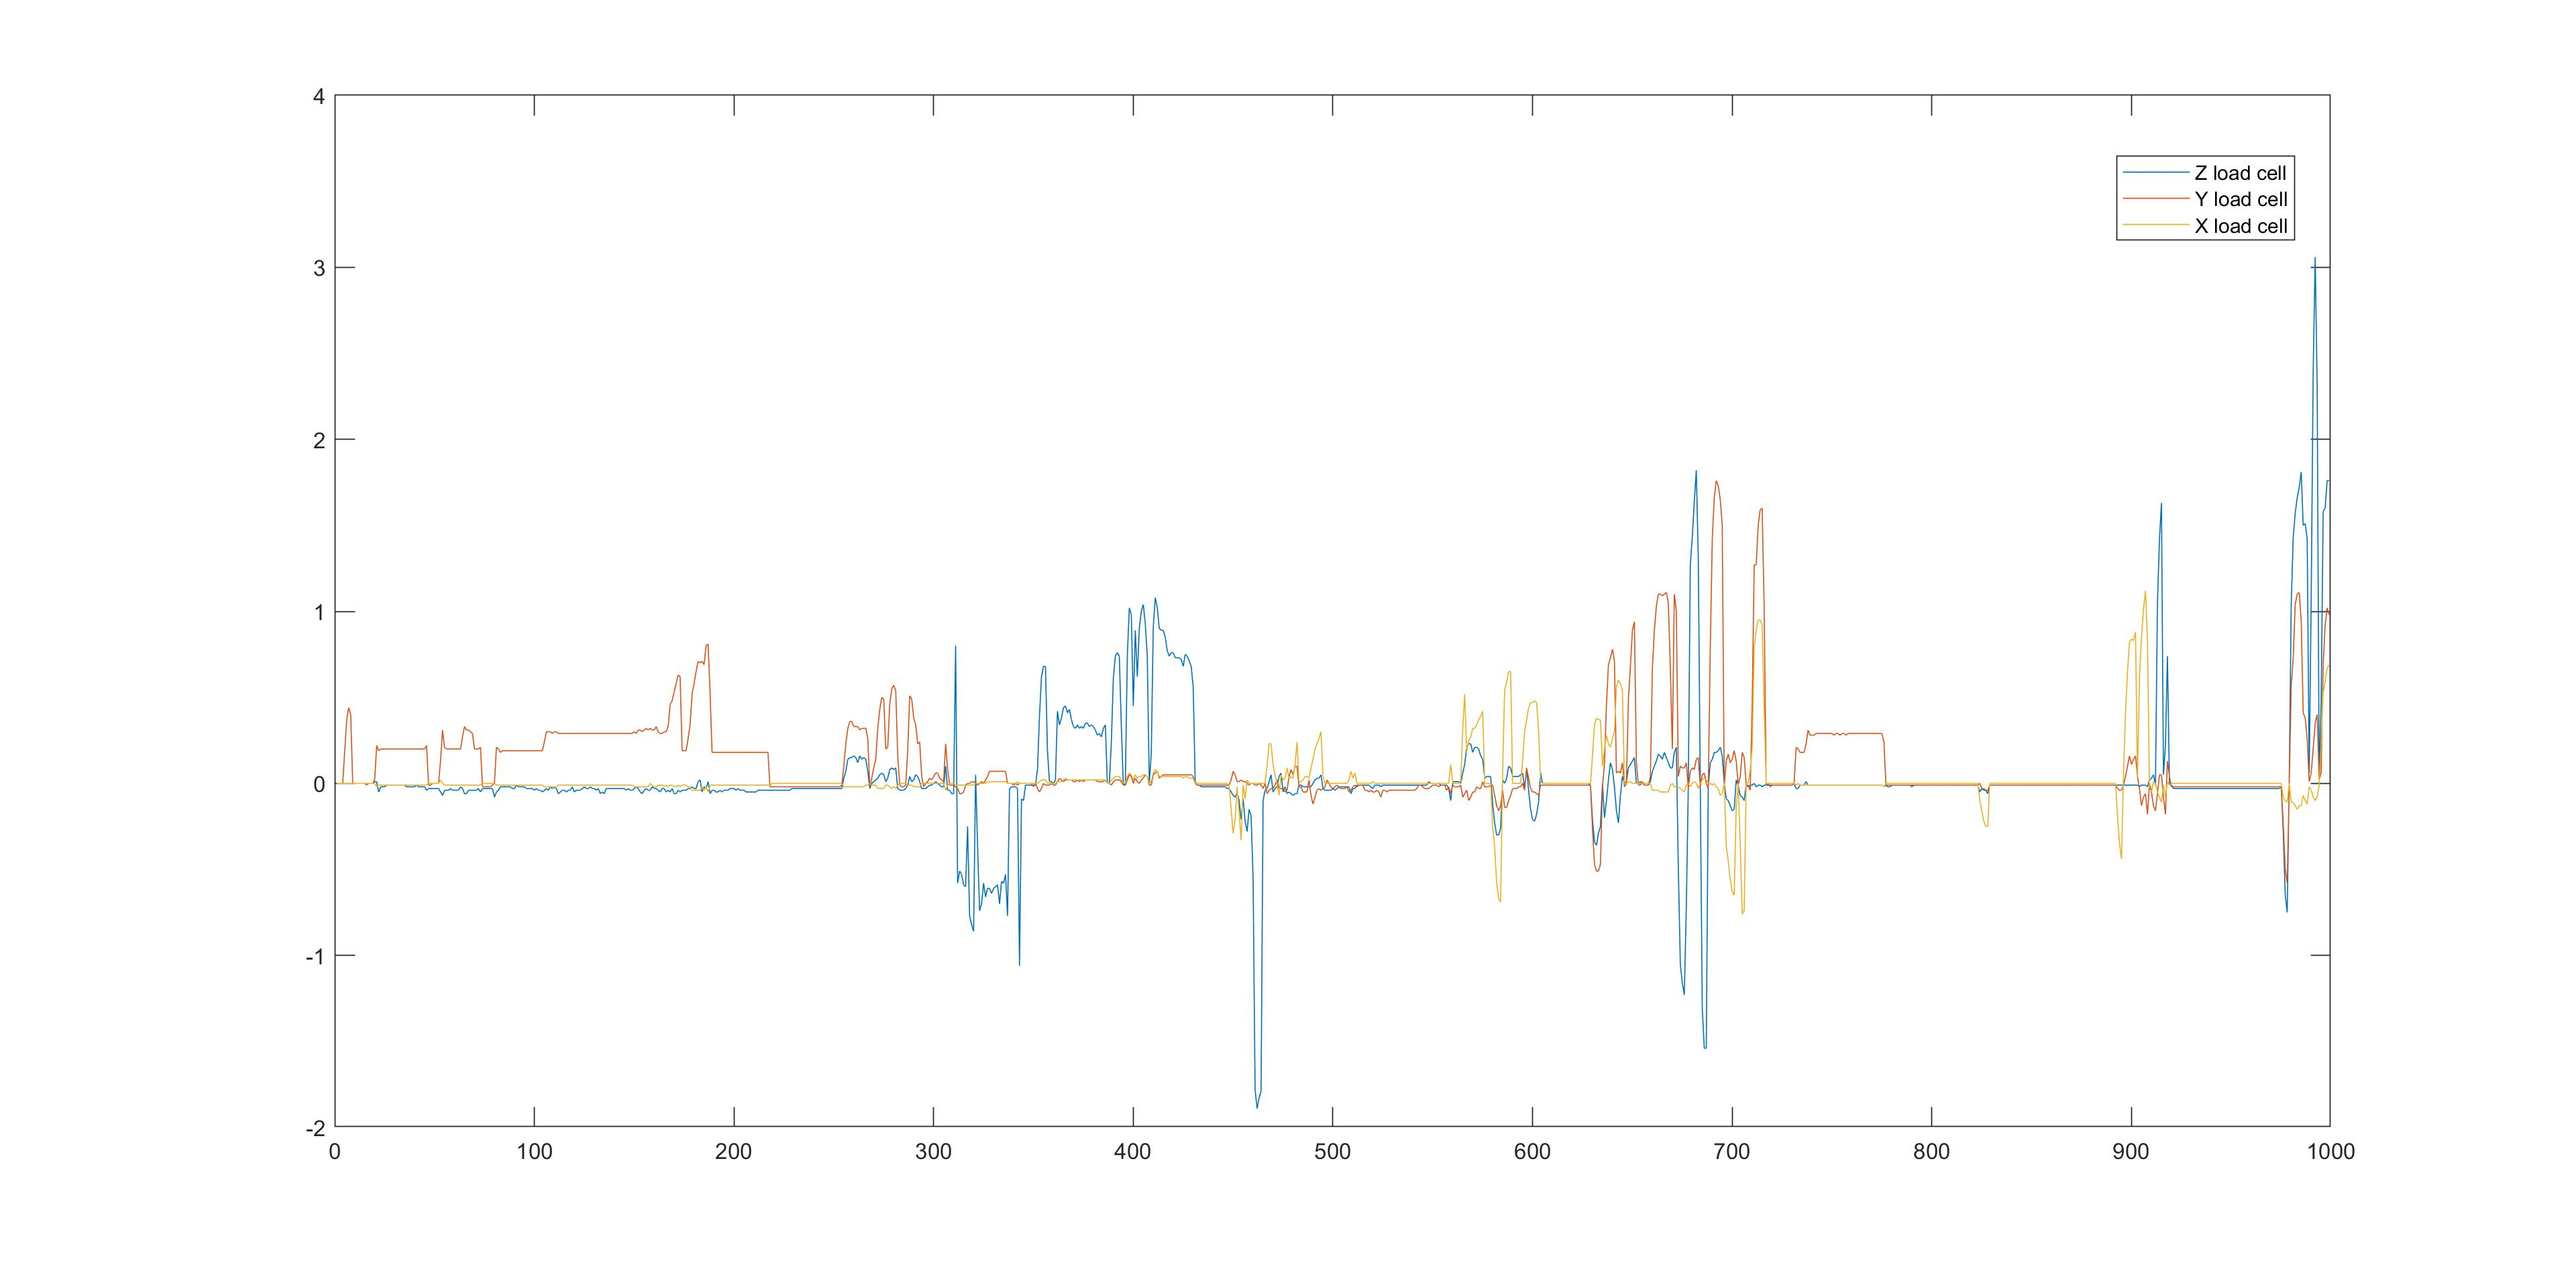
\includegraphics[width=1.2\linewidth]{figures/ch4/matlabresult1}
	\caption{Figure showing one of the test}
	\label{fig:matlab1}
\end{figure}


\begin{figure}[p]%matlab result graph2
	\centering
	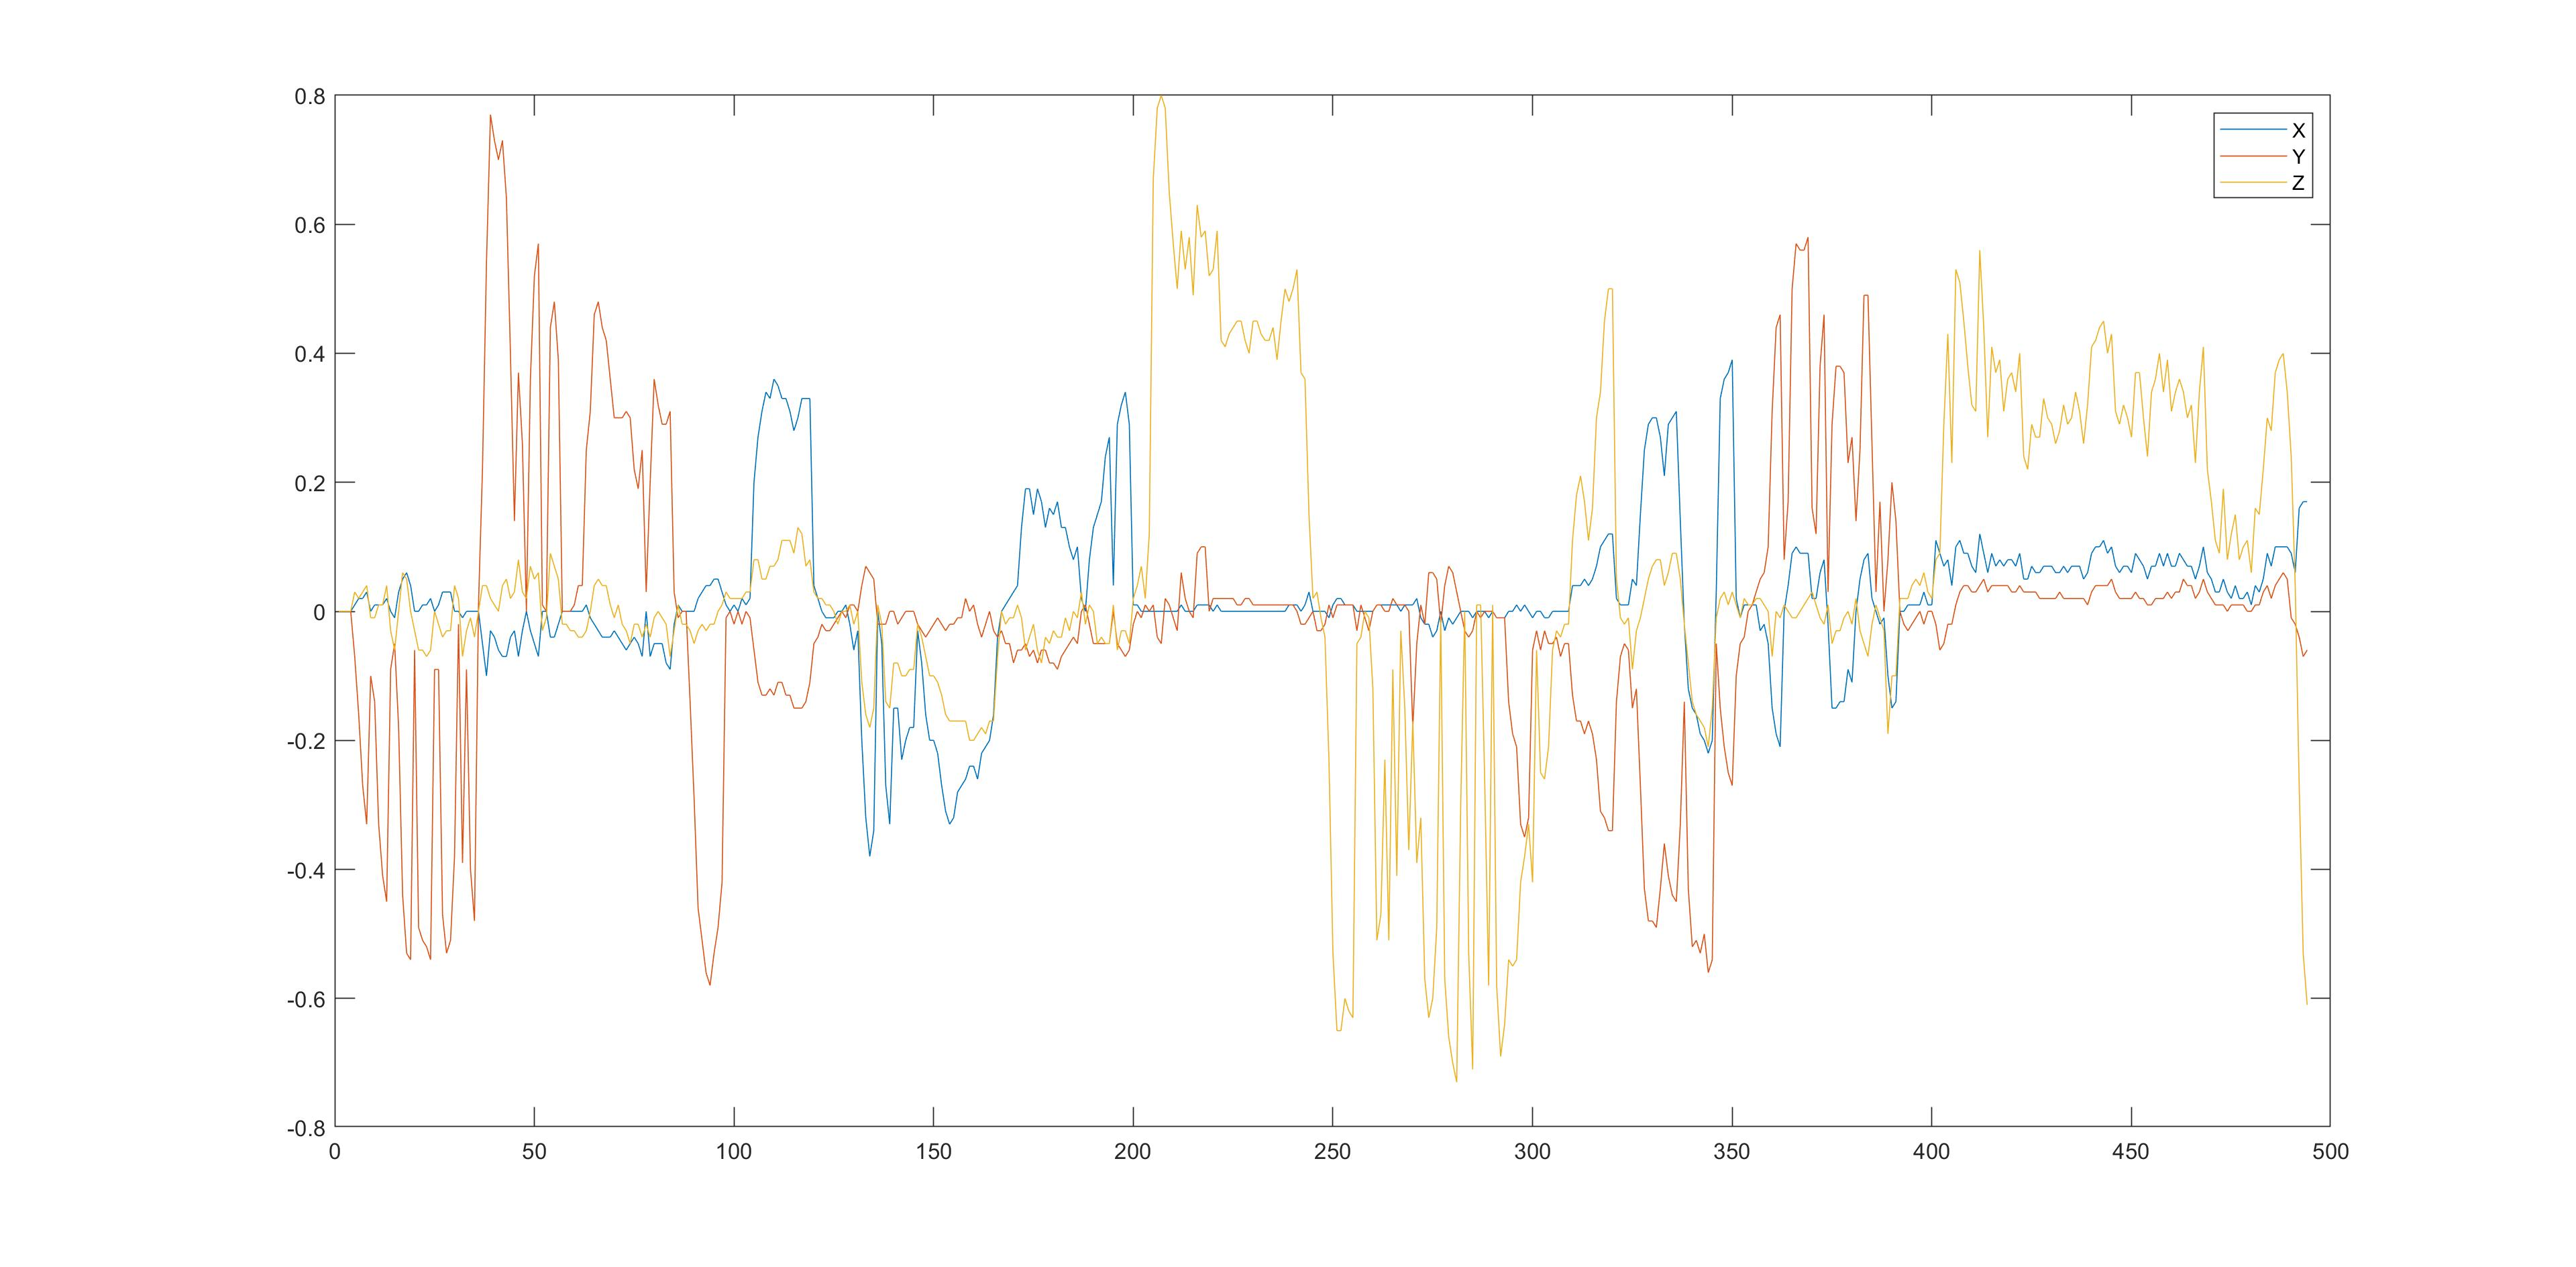
\includegraphics[width=1.2\linewidth]{figures/ch4/matlabresult2}
	\caption{Figure showing another test}
	\label{fig:matlab2}
\end{figure}

\section{Result of the \ac{blue} demonstration version}
The development version of \ac{blue} has been completed and is able to visually show a bilateral robot and a implementation of a hybrid control scheme combining a active assist and the master slave control scheme.\\
making use of the design: \ref{fig:bluepres}, and the code: \ref{code:arduinomaster} in combination with a python gui code and physical structure is completed and able to be used.

\section{Conclusion of Transfer Learning approach}
Transfer learning is a broad area with multiple methods that can be implemented to solve a problem that requires the use of transfer learning.\\
the first choice to use was the inductive transfer, followed by transductive, both methods failed to be suitable for implementation due to the fact that they are methods only for classification tasks. Since the problem in question to be solved, i.e. the prediction of values from a force sensor is a regression problem, this requires a regression transfer learning method, and the best method that can be used is found to be a transductive inference method which uses the transductive method but for a regression problem.\\
Therefore the best method for solving the problem of transferring knowledge to reduce calibration times of a force sensor array is the transductive inference.
\section{Discussion}
\subsection{Discussion of Force-sensor results}
From the small data collected from the novel force-sensor shown in Figures \ref{fig:matlab1} and \ref{fig:matlab2}. it can be seen that the novel force sensor system is a usable multi-axis sensor with a lot of co-linearities which can be reduced with machine learning methods such as transfer learning methods in the future.
		\chapter{Conclusion} \label{Ch:5}
	
\section{Introduction} \label{sec:Introduction5}
The growth of wireless communication networks has led.			
		%\chapter{Conclusion and Future Works}\label{Ch:6}
Wireless communication  networks designers and operators are faced with the ever-increasing demands for wireless radio network resources and improved QoS provisioning. These challenges are driven by the always best connected (ABC)  access network  demands through network selection by wireless network users,  constant connectivity at anywhere demands by users and the explosive growth of multimedia-hungry devices, such as smartphones, tablets,  etc. within the wireless communication networks. Efficient radio resource utilization and QoS provisioning are major issues for wireless communication networks. \par 

 In this thesis, the use of MCDM algorithm, call admission control scheme, and cooperative communication techniques to improve the ABC network experience, enhance the radio resource utilization, and QoS provisioning for wireless network users are explored. Section \ref{sec:SummaryofContributions6}  gives the summaries of thesis's contributions. Finally, Section \ref{sec:FutureWork6}  highlights some important directions for future work.
 
\section{Summary of Contributions} \label{sec:SummaryofContributions6}
 In Chapter \ref{Ch:1}, an overview of current  challenges in radio resource management  of wireless communication networks is provided. The chapter introduces the research problems addressed in this research work, the motivations, the research questions, and  research objectives. In addition, the research contributions and scope, as well as the outline on the thesis organization are also provided. In Chapter \ref{Ch:2}, the background topics for the thesis the is presented. \par
 
Chapter \ref{Ch:3}  studied the problem of enhancing QoS for wireless  MoH  based cellular networks. An  ATMA  CAC algorithm is proposed. The ATMA CAC  exploits the knowledge of the  calls generation pattern and  moving phase and stationary phase events of the MoH networks to enhance the new call blocking probability, handoff call dropping probability, and channel resource block utilization of the moving wireless networks. The  ATMA scheme adaptively smoothens out the new calls, depending on the mobility events of the HSRC. A  framework to investigate the effect of varying  load traffic on the new call blocking probability, handoff call dropping probability, and resource block utilization of the proposed scheme  using Markov chain analysis is developed.  The simulation results demonstrated that the ATMA  CAC scheme  improved  resource block utilization; with reduced new call and handoff call dropping probabilities compared to NMAT  CAC scheme.  \par 
 
Chapter \ref{Ch:4}  investigated the problem of throughput and QoS enhancement in wireless cellular networks with cell-edge users. A BCC scheme that  opportunistically  engage UES in cooperative communication and  exploits the transmission channel qualities variation with adaptive modulation coding to enhance the average throughput, QoS, and radio resource utilization in the cellular wireless  networks is proposed.  An analytical framework, using Markov chain process to investigate the effect of the queue buffer size on the average throughput, call  blocking probability, and radio resource utilization under varying inter-arrival rates (network  load),  UE cooperative relay  and cell-center zone  indice of the wireless networks is developed. A platform to investigate the benefit/gain performances of the  BCC scheme for improving the network bit-rate transmission, radio resource utilization, and blocking probability of  UEs' compared to NBCC scheme is provided. The simulation results showed that the proposed BCC scheme achieved a significant improvement in the average  throughput,  data blocking probability, and radio resource utilization for wireless communication networks compared to the NBCC scheme. \par 
 
In Chapter \ref{Ch:5},  the problem of access network selection  for single and group calls in HWNs is investigated.  The application of a new MCDM algorithm named  MULTIpliative Multi-Objective Optimization Ratio  Analysis (MULTIMOORA) for VHO in HWNs and compared it with some traditionally popular  MCDM schemes: SAW, GRA, VIKOR, and TOPSIS.   A detailed performance evaluation of the proposed scheme  was conducted for single calls.  The results demonstrate that MULTIMOORA outperformed SAW, GRA, and VIKOR in terms of access network selection for single calls (voice, file-download, and video-streaming), while having similar access network selection performance with TOPSIS for the  access  network's single call  traffic considered. 



The access network selection for group calls in HWNs with dynamic criteria investigations  demonstrated that TOPSIS algorithm utilizes the  benefits of  WLAN more than MULTIMOORA algorithm  at low speed, while MULTIMOORA algorithm  utilizes the benefits of LTE more than TOPSIS algorithm  at above low speed region for both high priority file-download and video-streaming group calls.   The  performance of TOPSIS is observed to be relatively more unstable at the high speed\textendash region, unlike MULTIMOORA's.
 The relative stability of MULTIMOORA comes from the reinforcement and integration of the  three decision making techniques of the MULTIMOORA. Furthermore from these findings, it can be suggested that  an  hybrid algorithm between MULTIMOORA and TOPSIS could produce an improved  access network selection algorithm for NGWNs.


 
\section{Future Work}\label{sec:FutureWork6}
 
 \subsection{Handover management in MoH networks} \label{subsec:MobileHotspot}
The NGWNs, such as 5G networks are proposed to be ultra-dense heterogeneous wireless communication networks.  Handover management in high mobility wireless network systems is still a major challenge that calls for further investigations. The seamless and efficient handover between different MeNBs and RATs remain an open area for future research.

 \subsection{ MoH networks with traffic load predictions} \label{subsec:loadPredictionMobileHotspot}

The wireless environment of practical MoH  networks is very dynamic. Some statistical characteristics of the MoH networks,
such as new arrival rate, handoff call arrival rates, and call lifetime  are time-varying. In MoH wireless network environment where  
these traffic load parameter values are not well known, the CAC algorithm  of  such MoH networks could be plagued  with inefficient management of the radio resources. An interesting solution to this problem would be to exploit network traffic load  predicting techniques.  Predicting techniques,  such as  Least Squares algorithm, Machine learning algorithm, Grey predictor scheme, would allow the mobile hotsot network to obtain the statistical parameters (call arrival rate and call life time) without prior knowledge. Hence, the investigation into the performance of MoH networks  with and without traffic load prediction scheme would  be an interesting extension for future work.



 \subsection{ Security of BCC }\label{subsec:Securityofbufferedcooperativecommunication}
In the BCC scheme,  it is possible for malicious relaying UE nodes to attack the network. Some UEs can possibly behave in a malicious manner by intentionally trying to corrupt the communication by sending  garbled signal to the  destination.  This action of  malicious relaying UEs can degrade the performance of the network.  Considering the effect of malicious  of relay  UE nodes attack and how to mitigate their actions  for ensuring the reliability the networks will be of  significant future research importance. 





 \subsection{ Inter-cell-interference in cellular  network communication with BCC deployment}
 
 In cellular wireless communication  networks, Inter-cell-Interference (ICI) is a predominant problem, especially among cell-edge UEs.  ICI problem can significantly degrade the QoS experience of the cell-edge UEs. The effect of the problem of ICI on the QoS experience for edge-cell UEs  in wireless cellular networks could  be worsen, with the deployment of 
  BCC network scheme, where  
 cell-center UEs  are engaged  opportunistically as relay nodes. Therefore, as future work  there be would  the need to investigate/examine the impact of BCC on ICI management in cellular communication networks, by comparing  the ICI performance of  cell-edge networks with BCC deployment and with NBCC deployment.
 
 
 
 
 
 \subsection{Access network selection}\label{subsec:Networkaccessselection}
The number of available access network alternatives within  HWNs can sometimes  fluctuate. One or more RATs can breakdown, and  its or their services become unavailable within the HWNS. Sometime more RATs can become activated, thereby increasing the number of available access networks within the HWNs. These variations have  been reported to affect the access network selection decisions of  MCDM  algorithms leading to   rank reversal/abnormality.  Further work should investigate  the rank reversal/abnormality and  sensitivity analysis  of performance of  MULTIMOORA compared to  TOPSIS.  Also, the interaction of criteria influence using ANP needs to be  investigated.
 
  
			% uncomment this line if you have chapter 6		 
		
		     
		         
		%%%%%%%%%%%%%%%%%%%%%%%%%%%%%%%%%%%%%%%%% APPENDIX - OPTIONAL - COMMENT IF NOT NEEDED %%%%%%%%%%%%%%%%%%
		\makeAppendixPage   %%% make the appendix title page - can be edited in ut-thesis-template.tex
		\appendix
		%\addToTOC{Summary of Equations}
		
\chapter{Additional Materials}\label{ch:litrev}
%\appendix
\section{Codes Used for this project}
\subsection{arduino code for reading forces from 3 load cells}


%arduino code c
\lstinputlisting[language=C,caption={Ardunio code used for data collection},breaklines=True,captionpos=t,label=code:arduinomaster]{codes/3_load_cell.ino}

\subsection{arduino code to implement the hybrid active master-slave control}

%arduino code c
\lstinputlisting[language=C,caption={Ardunio code used for data collection},breaklines=True,captionpos=t,label=code:arduino]{codes/v1.ino}

\subsection{arduino code for calibrating each of the load cells}

%arduino code c
\lstinputlisting[language=C,caption={Ardunio code used calibrating each loadcell},breaklines=True,captionpos=t,label=code:calibration]{codes/calibration.ino}

\newpage


\subsection{python code for collecting data and storing it}
%pyton code listing not figure
\lstinputlisting[style=python,language=Python,caption={Python code used for data aquisition},breaklines=True,captionpos=b,label=code:py]{codes/force_torque.py}\newpage
\restoregeometry
\newgeometry{left=0.2cm,right=0.2cm,bottom=0.5cm} 
\section{Literature Review on Existing Bilateral Robots}\label{sec:bilatrob}
\href{https://docs.google.com/document/d/1uwM2z0r_MtfIO8P_6Rdd-_3ZBnt-zjLi/edit?usp=sharing&ouid=106338247166493930992&rtpof=true&sd=true}{link to full literature review}

\begingroup
\linespread{0.9}\sffamily\footnotesize
\begin{longtable}{|p{4cm}|p{3.8cm}|p{7cm}|p{4cm}|}
	\caption{Literature Review of Bilateral Rehabilitaion Robots}
	\label{tab:reviewbilateral}\\
	\hline	Overview&Aim&Methodology&Results\\
	\hline\hline
	\endfirsthead
	%&&&\\
	%\hline	
	\hline Overview&Aim&Methodology&Results\\
	\hline\hline
	\endhead
	An assessment of robot-assisted bimanual movements on upper limb motor coordination following stroke \cite{Lewis2009}. &The purpose of this study was to quantify the influence of
	robot-assisted bimanual movement on the timing of muscle activity
	and limb-robot interface forces during arm reaching tasks
	performed by individuals with hemiparesis.
	&15 subjects with poststroke hemiparesis, with all having suffered a \ac{cva} at least 12 months prior and had residual unilateral deficits in upper limb function. participated in 2 separate data collection sessions, they performed unimanual paretic limb, unimanual nonparetic limb and bimanual condition under each session. In the bimanual condition the task was performed in a mirror image symmetric manner.
	&For the first goal, when movement was specified by the nonparetic arm, force and emg profiles showed that the initial muscle activation was more synchronized with the limb motion during bimanual, robot-assisted movement.
	For the second goal, force and muscle activation profiles were similar in voluntary and robot-assisted bimanual movement. 
	Showing that bimanual robot-assisted movement training could provide additional therapeutic benefits beyond those of unimanual robot-assisted training in the long term.\\
	\hline
	Bilateral assessment of functional tasks for robot-assisted therapy applications \cite{Johnson2011b}.&To present a novel evaluation system along with methods to evaluate bilateral coordination of arm function on activities of daily living tasks before and after robot-assisted therapy&In the first study 10 healthy and 7 stroke subjects were included, with the stroke subjects having had a stroke occurring >6 months prior. While in the second study 4 stroke subject were included. 
	\ac{uefm} was used to describe motor control in the impaired arm, and the \ac{ueft} was used to describe functional disability levels.
	&It was found that the bias was able to measure accurately right and left arm kinematics during typical functional tasks and quantify movements during functional tasks pre- and post-robot therapy.
	Results from both studies showed the \ac{bias} system can accurately measure the kinematic wrist positions of all subjects regardless of impairments levels.\\
	\hline
	Rehabilitation robot with patient cooperative control for bimanual training of hemiparetic subjects \cite{Trlep2011}&To study the developments and validation of a bimanual training system that stimulates the use of both arms of the hemiparetic subjects.&The system is based on the HapticMaster, it is an admittance-controlled robot manipulator with a control loop rate $2500hz$ and consists of 3 active \ac{dof}, it was expanded with an extra joint to allow simulation of an active steering wheel which are bimanual handlebars mounted on the robot end-effector, and forces generated by each arm is measured by 2, 6- \ac{dof} force and torque sensors, a passive gravity compensation mechanism was implemented to compensate the weight of the subject’s upper extremities.&After the pilot study with 4 subjects with 8 trainings.
	The paper presents a system for unimanual and bimanual training and the system can be used as an evaluation device to monitor the patients progress and level of motor functionality.\\
	\hline
	Robot-assisted arm trainer for the passive and active practice of bilateral forearm and wrist movements in hemiparetic subjects \cite{Hesse2003}&To determine whether use of a robotic arm trainer for bilateral exercise in daily repetitive training for a 3-week period reduced spasticity and improved motor control in the arm of the severely affected, chronic hemiparetic subjects&The arm trainer was designed to allow the bimanual practice of a 1df pronation and supination movement as well as dorsiflexion and volarflexion of the wrist of the forearm, 3 operational modes were programmed which are passive mode with speed and \ac{rom}, active mode with mirror control and active mode as previous but the paretic arm has an isometric resistance to overcome.
	The trainer drivers can provide torques of up to 5Nm, a display shows the number of performed cycles.
	&The subjects had a positive impression on the therapy, and they reported that muscle tone reduction lasted a day. The end of the practice with the trainer resulted in a sustained reduction of muscle tone in most of the subjects and motor function improved in 5 of the subjects.\\
	\hline
	Incorporating haptic effects into three-dimensional virtual environments to train the hemiparetic upper extremity \cite{Adamovich2009}&Describes the design and feasibility testing of a robotic/virtual environment system designed to train the arm of persons who have had stroke.&The system makes use of a Haptic master a 3-dof admittance-controlled robot, a 3-d force sensor measures the external force exerted by the user also the velocity and position of the robot are measured at 1000hz and are used to generate reactive motion based on the properties of the virtual haptic environment. The \ac{haapi} allows the robot to programmed to produce haptic effects.&There was an improvement in the smoothness of the trajectories in all subjects.
	2 subjects improved their aggregate time to complete all 15 timed items.\\
	\hline
	Upper-limb powered exoskeleton design \cite{Perry2007}&To define the kinematics and dynamics of the upper limb during daily living activities to develop a anthropomorphic 7-\ac{dof} powered arm exoskeleton.&A preliminary study was carried out to understand the kinematic and dynamic requirements of an exoskeleton arm for functional use. Motions of the human arm was recorded during 18 \ac{adl} tasks which were divided into the following categories, general reaching tasks, functional tasks, eating and drinking, hygiene related tasks. &A robotic exoskeleton system was developed and tested using new techniques.\\
	\hline
	Computerized arm training improves the motor control of the severely affected arm after stroke a single randomized trial in two centers \cite{Hesse2005}&To compare a computerized arm trainer and electromyography-initiated electrical stimulation of the paretic wrist extensor in severely affected subacute stroke patients.&44 Subjects who had a stroke interval of 4 to 8 weeks were recruited to participate in the trial, the subjects practiced with an \ac{at} or \ac{es} with their paretic wrist extensors for 20minutes every day for 6 weeks. &There was improvement in the \ac{fms} for both groups, but significantly more in the AT group.\\
	\hline
	Repetitive bilateral arm training with rhythmic auditory cueing improves motor function in chronic hemiparetic stroke \cite{Whitall2000}&Investigation to determine if \ac{batrac} will improve motor function in the hemiparetic arm of stroke patients.&16 patients were recruited, they all experienced stroke >12 months previously. The training consisted of 20 minutes on the \ac{batrac} 3 times per week for 6 weeks.&14 patients completed the protocol and the \ac{uefm} showed significant improvements, only 3 subjects could extend their finger joints by >10degrees and wrist by \>20 degrees.\\
	\hline
	Driver’s SEAT: \ac{seat} \cite{Johnson1999}&Describes the design and philosophy of Driver’s \ac{seat}, a 1-dof robotic device that aims to promote coordinated bimanual movement.&The system consists of a motor, an adjustable-tilt, split steering wheel, a height adjustable frame, wheel position sensor, force sensors, \ac{sti} simulation hardware and experimenter computer.&It is a system designed to be used to stroke subjects with either right or left hemiplegia and was used in on 8 stroke patients.\\
	\hline
	Bilateral movement training with computer games for stroke rehabilitation \cite{King2010}&This paper describes two devices developed to use computer games during bilateral arm training.&Movement assisted gaming system is developed where the user sat with their arms strapped onto forearm supports and their hands rested on a joystick or palmar supports. &All the subjects reported they enjoyed using the device, and some described how their functional activity had improved.
	And from the \ac{fms} it was found that there was no deterioration because of the intervention.\\
	\hline
	Robotic stroke therapy assistant. \cite{Mahoney2003}&Describes the Design considerations and clinical outcome with regards to the phase 1 system of the \ac{arcmime}.&The \ac{arcmime} is made to be able to carry out the 4 control modes of the \ac{mime} system which are passive, active-assisted, active-constrained and bimanual mode. &There was no statistical difference between the \ac{arcmime}, and\ac{mime} forces directed toward the subjects. The subject feedback was neutral between both robots\\
	\hline
	A robotic system for upper-limb exercises to promote recovery of motor function following stroke. \cite{Lum1999}&To evaluate the therapeutic efficacy of robot-aided exercise for recovery of upper limb motor function following stroke.&Chronic stroke patients with \>6 months post \ac{cva} and were assigned randomly into either control or robot group, and they receive 24 one-hour sessions over 2 months.&The robot group subjects exhibited decreased resistance to some passive movements and improved performance of some active-constrained reaching movements post-treatment.
	Preliminary data from the ongoing clinical trial suggests robot-aided exercise has therapeutic benefits which can been seen improvement in active-constrained training tasks and the\ac{fma} of motor function.\\
	\hline
	Rhythmic bilateral movement training modulates corticomotor excitability and enhances upper limb motricity poststroke: a pilot study. \cite{Stinear2004}&To investigate whether repetitive bimanual coordinated movements enhanced upper limb corticomotor excitability and motor function poststroke.&9 poststroke patients ranging from 2 to 84 months post stroke were recruited; grip strength wrist flexor and wrist extensor forces were assessed before each mapping session.&5 patients increased their motricity scores over the period of the intervention.
	The experimental findings support the predicted increase in motricity and changes in Cortical maps excitability in response to \ac{apbt}. And there was no evidence that one of the 2 movement patterns were more effective than the other.\\
	\hline
	Priming the motor system enhances the effects of upper limb therapy in chronic stroke. \cite{Stinear2008}&To examine the effects of \ac{apbt}.&32 subjects, having had stroke 6 months prior were recruited and divided into either control or \ac{apbt} group. All subjects were given a set of wooden blocks to use for their intervention for which they had to pick up and transport the block 20cm. the \ac{apbt} group made use of a \ac{apbt} device for 15 mins.&All subjects were stable at baseline and improved immediately after intervention, but only those primed with \ac{apbt} before motor practice showed sustained improvement in upper limb motor function.\\
	\hline
	The \ac{mime} robotic system for upper-limb neuro-rehabilitation results from a clinical trial in subacute stroke. \cite{Lum2005}&Presents the results from a randomized, controlled clinical trial of the \ac{mime} robotic device for shoulder and elbow neurorehabilitation in subacute stroke patients.&The paretic arm was strapped to reduce wrist and hand movement, the Puma 560 robot is attached to the splint, there are 4 modes of robot-assisted movement.
	Subjects had a \ac{cva} 1-5 months prior, intervention consisted of 1 hour treatment 15 times, the robotic treatment used was similar to a previous study and there were 3 groups for this study, robot-unilateral, robot-bilateral, robot-combined and control group. 
	Robot-unilateral group performed 
	Subjects were tested before and after each assignment the FM assessment
	&Both robot groups had significant gains in the proximal and distal \ac{fms}, \ac{mss} movement, motor power and \ac{fim}. 
	The robot-combined group had a better Ashworth score compared to the robot-unilateral group.
	Compared to the control group the robot-combined group had greater gains in the proximal \ac{fms} and \ac{mss}, and the control group did better than the robot-unilateral group.
	The robot-bilateral group did poorer on motor power and \ac{fim} compared to the robot-unilateral and control groups.\\
	\hline
	Development of robots for rehabilitation therapy: the palo alto VA/Stanford experience. \cite{Burgar2000}&To summarize the development and clinical testing of 3 mechatronic systems for post-stroke therapy.&The 3 mechatronic system discussed are upper limb patient-controlled manipulation orthosis, \acf{mime} and a third gen version of the \ac{mime} system.&\\
	\hline
	Robot-assisted upper-limb therapy in acute rehabilitation setting following stroke: Department of Veterans Affairs multisite clinical trial. \cite{Burgar2011}&To evaluate whether the \ac{mime} can facilitate similar or greater motor recovery as the same of early hands-on therapy &54 Subjects entered the study between 7-21 days after stroke. Divided into 3 groups, robot low does, robot high does and control. Control and robot low receiving 15 1 hour sessions over 3 weeks and robot high receiving 30 1 hour sessions over 3 weeks. &At post treatment the robot-hi and control groups had higher \ac{fms} than the robot-lo group with both groups showing similar results. But at the 6 months follow up the robot-lo and control group results were similar but the robot-hi results much higher than both, and the robot-lo group showing large improvements compared to both groups.\\
	\hline
	Bilateral upper limb trainer with virtual reality for post-stroke rehabilitation: case series report. \cite{Sampson2012a}&To investigate the body function effects and motivational effects of a combined therapy based on several stroke rehabilitation concepts.&The system comprises of the \ac{built} with \ac{vr}, the \ac{built} facilitates bilateral movement in the horizontal plane of the affect arm, forearm supports are used to hold the upper limb in places and allow the patient to grip with a joystick style grip on the handle. The BUiLT provides shoulder and elbow flexion/ extension, shoulder adduction/ abduction, external/internal rotation, and combined movement patterns.&The results showed increase in \ac{uefm} scores across all subjects, there was also increase in joint movements in most of the subjects.
	Overall, the results from the intervention shows there was a trend of positive effect on UL function from the \ac{built} + \ac{vr}. Isometric strength also showed a mostly increasing result across all the subjects.
	The question form results indicate that the system highly motivated the subjects to exercise, and they were able to complete the full regiment.
	\\
	\hline
	Robot-assisted movement training compared with conventional therapy techniques for rehabilitation of upper-limb motor function after stroke. \cite{Lum2002}&To compare the effects of robot-assisted movement training with conventional techniques for rehabilitation of the upper-limb motor function after stroke.&This paper makes use of the \ac{mime} system. 30 Subjects were enrolled in study if they had a diagnosis of a single \ac{cva} and were more than 6 months post \ac{cva}. Subjects were assigned to control or robot group, each group received 24, 1-hour treatment sessions over 2 months.
	The robot group emphasis was on targeted reaching movements, while for the control was on re-education of muscles using a sensorimotor approach to control motor output.
	&Compared with conventional treatment of equal intensity and duration, the robot-assisted movements had advantages after 2 months of treatment in terms of decreasing impairment, improving strength and increasing reach extent.\\
	\hline
	Machines to support motor rehabilitation after stroke: 10 years of experience in Berlin. \cite{Hesse2006}&Presents the devices and related clinical studies for the motor rehabilitation of these upper limbs.&\textbf{Bi-Manu-Track}: it is a 2x1 \ac{dof} than enables hemiparetic patients to bilaterally practice 2 different movement cycles, forearm pronation/ supination and wrist flexion and extension. &The robot-trained group had superior results at the end of the study and at a 3-month follow up\\
	\hline
	Unilateral and Bilateral upper-limb training interventions after stroke have similar effects on bimanual coupling strength. \cite{VanDelden2015}&To determine whether the degree of coupling between both hands is higher after bilateral than after unilateral training. &60 subjects were admitted into the trial with an average time after stroke of 9.3 weeks and divided into 3 groups \ac{mcimt} which is the unilateral group and involved unilateral repetitive tasks, modified \ac{mbatrac} and dose matched control treatment. All subjects received 1-hour therapy sessions 3 days per week for 6 weeks.
	The study makes use of 4 tasks which are bimanual coordination task, kinesthetic tracking tasks, unimanual motor task and unimanual reference task.
	&At the follow-up, the \ac{dmct} group showed significantly stronger intended coupling in the in-phase kinesthetic tracking test than at post intervention.
	There was observed improvements in the paretic hand movements after \ac{mbatrac}.
	\\
	\hline
	Comparing unilateral and bilateral upper limb training: the \ac{ultra}-stroke program design. \cite{VanDelden2009}&Describes the design of a single-blinded randomized clinical trial to access the effectiveness 2 new intervention techniques in subacute stroke patients and to examine the changes in how sensorimotor functioning relate to changes in stroke recovery mechanisms.&This paper makes use of both \ac{batrac} and \ac{cimt}. 
	60 subjects were recruited with the criteria of having a CVA within 6 months. The trail is to last for 6 months.
	The \ac{mbatrac} group receives 1-hour sessions, 3 days a week for 6 weeks. A computer is connected to the potentiometers on the devices measures movements and provides feedback, this computer is also used to start each exercise. &No significant difference between groups on the primary and secondary outcome measures between groups at posttest ad follow-up. All groups demonstrated significant improvement on the action research arm test after intervention during the 6 weeks follow up\\
	\hline
	Quantifying learned non-use after stroke using unilateral and bilateral steering tasks. \cite{Johnson2011}&To examine whether the behaviour of underutilizing the impaired arm slowing down re-acquisition of bilateral coordination can be studied and quantified using the TheraDrive.&The TheraDrive is used as the experimental apparatus for the study, the system consists of a Logitech force-reflecting wheel mounted on a height adjustable metal frame, the drive is connected to a UniTherapy software platform that records the angular movement of the wheel.&The results showed higher average errors for the impaired arm tracking than non-dominant arm tracking, confirming it is not as efficient in performing tracking tasks when compared to the dominant arm in stroke survivors.
	And it was also found that when the paretic arm is highly involved the performance of bilateral tracking tasks will be affected and bilateral tracking errors will be like unilateral tracking errors with the impaired arm.
	\\
	\hline
	Experimental results using force-feedback cueing in robot-assisted stroke therapy. \cite{Johnson2005}&To evaluate a novel force-feedback and reinforcement strategy aimed at limiting the tendency of stroke survivors with hemiparesis to overuse their less-affected arm.&8 subjects participated with a mean time after stroke of 4.8 years. The Drivers \ac{seat} system was used for this study. \ac{semg} activity for the 7 upper limb muscles were recorded. 
	There were 4 conditions data was obtained from the wheel which are: N-bi, A-bi, N-WA, A-WA. 4 trials were completed for each steering task. Subjects were tasked to track a target on the screen while steering through 15 RT, ST and LT segments on the track.
	All subjects had data collected for the 4 modes and the data was used to evaluate the effect of the corrective force
	& Corrective force cues had some effect on the weak arm participation rate of all subjects during bilateral steering of the preview track.
	It was found that a significant force cue effect on the impaired arm of subjects during particular movements in one therapy session with the device, indicating that the subjects used their impaired arm differentially in each of the force-cue condition
	\\
	\hline
	Bilateral arm training with rhythmic auditory cueing in chronic stroke: not always efficacious. \cite{Whitall2000}&To determine whether the reported results from a modified form of \ac{batrac} could be replicated.&15 Subjects participated in the trial had a stroke at least 6 months prior. The \ac{uefm} was used for assessment.
	The intervention involved the subjects moving the \ac{batrac} for 5 minutes with 10 minutes break. And this was done for 2 weeks with 2.25-hour sessions.
	&It was found that an increase in training speed did not have a consistent effect on functional outcomes but contributed to perceived ability and use of ability. 
	A larger proportion of subjects with left hemisphere damage responded on the \ac{uefm} and \ac{wmft} scales.
	It was found for subjects with lower initial \ac{uefm} their gains were much larger than the other group
	\\
	\hline
	25 post stroke shoulder-elbow physiotherapy with industrial robots. \cite{Toth2006}&Describes the REHAROB therapeutic system.&2 ABB industrial robots were selected for delivery of exercises, with one connected to the upper arm and the second to the lower arm. A Orthosis is developed to connect the patient’ upper and lower arm to robot, it is of an exoskeleton form.&With the \ac{mas} scoring there was improvement in both shoulder adductors and elbows flexors in all but 1 subject. The range of motion of all subjects increased at the end of the trial same with the \ac{fim} and Barthel index.
	it was also found that the patients were not afraid of the robot and the therapists were able to learn how to use the system, and the system was working reliably.
	\\
	\hline
	Effects of robot-assisted upper limb rehabilitation on daily function and real-world arm activity in patients with chronic stroke: a randomized controlled trial. \cite{Liao2012}&To compare the outcome of robot-assisted therapy with dose matched active control therapy using accelerometers to study functional recovery in chronic stroke patients&20 subjects were recruited for the study, all having a \ac{cva} after 6 months. Subjects were randomly assigned to robot-assisted therapy or to dose matched active control therapy.&There were significant benefits of the robot-assisted therapy compared to the active control group on the amount and quality of functional arm activity for the hemiplegic hand in the living environment. 
	This study demonstrated that an accelerometer could be a suitable measure of treatment efficacy in robot-assisted therapy. Also showed that robot-assisted therapy combined with 15 minutes of functional activity has great benefits on real world arm activity
	\\
	\hline
	Kinematic data analysis for post-stroke patients following bilateral versus unilateral rehabilitation with an upper limb wearable robotic system. \cite{Kim2013}&This paper reports on a randomized clinical trial utilizing a complete robot-assisted rehabilitation system for the recovery of the upper limb function in patients’ post-stroke.&The \ac{ulexo} was used for this study.
	25 subjects joined the trial having passed the requirements of having a \ac{fms} between 16 and 39 and more than 6 months post stoke. They were randomly divided into 3 groups: unilateral robot training, bilateral robot training and usual care.
	&It was found that bilateral movement training delivered a better rehabilitation result to subjects except in the reaching exercise.
	The \ac{fms} showed that there is no significant difference between the 2 training methods.
	It was found that when considering individual evaluation metric that the bilateral training scheme delivered better rehabilitation result with respect to the wrist joint movement.
	\\
	\hline
	MIT-MANUS: A Workstation for manual therapy and training I. \cite{Hogan1992}&This paper presents some recent work on the development of a workstation for teaching and therapy in manual and manipulative skills.&The MANUS has 5 \ac{dof}, a direct-drive five bar linkage SCARA mechanism provides 2 translational \ac{dof} for the elbow and forearm motion. A differential mechanism driven by geared actuators provides 3 \ac{dof} of wrist motion: extension-flexion, abduction-adduction and pronation-supination.&The proposed system was built and tested in multiple future clinical trials\\
	\hline
	Combined transcranial direct current stimulation and robot-assisted arm training in subacute stroke patients: an exploratory, randomized multicentre trial. \cite{Hesse2011}&To test the combination of upper arm interventions were tested in a double-blind randomized trial.&96 patients were randomized for 6 weeks and split into 3 groups which received anodal stimulation, cathodal stimulation, and sham stimulation, respectively. The inclusion parameters were that the patients were at least wheelchair mobile and had a severe flaccid \ac{ul} paresis with minimal hand and finger extensor activity. &All patients improved their \ac{fms} significantly over time, and between-group differences did not occur at any time. 
	Contrary to the hypothesis, nether stimulation affected the bilateral robot-assisted arm training.
	\\
	\hline
	Guidance-based quantification of arm impairment following brain injury: a pilot study \cite{Reinkensmeyer1999}&Reports the design and preliminary testing of a device for evaluating arm impairment after brain injury.&4 control subjects with no known history of neurological deficits and 4 brain-injured subjects participated in the trial. The device to be used was the \ac{arm} guide that uses a custom splint that rides along a linear constraint. &The results support the hypothesis that abnormal synergies would manifest themselves as distinct patterns of constraint force during guided movement.\\
	\hline
	Upper and lower extremity robotic devices to promote motor recovery after stroke- recent developments. \cite{Schmidt2004}&This paper presents clinically viable devices for upper and lower extremity rehabilitation.&The upper rehabilitation device discussed is the Bi-Manu-Track robot, which enables the bilateral passive and active practice of 2 movements which are: forearm pro-supination and wrist flexion and extension in a mirror/ parallel way. &The study shows the viability of robotic devices in rehabilitation of both upper and lower limbs, with subjects involved the trails showing improvements.\\
	\hline
	Design and development of a hand robotic rehabilitation device for post stroke patients. \cite{Rashedi2009}&Describes the design of a robotic device for rehabilitation of upper limbs of post stroke patients.&The apparatus was designed to provide the passive or active unilateral or bilateral therapeutic exercises for the upper limb in 2 operation states. Pronation/supination of forearm and flexion/extension of wrist. A special form of handles allowed them to be used for both movements without the need to be exchanged.&The device was tested on a female patient with left sided paretic arm, who utilized all 3 modes, the device was able to produce an accurate mirror image position tracking of the master limb.\\
	\hline
	A new haptic workstation for neuromotor rehabilitation. \cite{Casadio2006}&It describes a new robotic workstation for neurological rehabilitation.&Solutions based on linear motor tables with non-reversible hears and typical robot designs based on kinematic chains were avoided to meet the requirement of back-drivability. &A prototype of the system was constructed, and the design assumptions were verified on it, and the authors are confident that it’s operational range is consistent with the typical human motions of the upper limb and it fit for robot therapy.\\
	\hline
	%&&&\\
	%\hline
\end{longtable}

\endgroup
\restoregeometry
\newgeometry{left=0.2cm,right=0.2cm,bottom=0.5cm}
\section{Literature Review on Clinical Trials of Bilateral Robots}\label{sec:clinical}


\begingroup
\linespread{0.9}\sffamily\footnotesize

\begin{longtable}{|p{3cm}||p{2cm}|c|p{3cm}|c|}
	\caption{Literature Review on Clinical Studies and their results}
	\label{tab:reviewclincal}\\
	\hline 	Paper and number & Number of patients & Stage of recovery & Range of weeks after stroke for recruitment & Use of FES \\
	\hline\hline
	\endfirsthead
	\hline 	Paper and number & Number of patients & Stage of recovery & Range of weeks after stroke for recruitment & Use of FES \\
	\hline\hline
	\endhead
	
	
	\cite{Lewis2009} & 15 & Chronic & $>$12 months & no \bigstrut\\
	\hline
	\cite{Johnson2011} & 11 & Chronic & $>$6 months & yes \bigstrut\\
	\hline
	\cite{Trlep2011} & 4  & Chronic & 5-13 years & no \bigstrut\\
	\hline
	\cite{Hesse2003} & 12 & Chronic & 6-16 months & no \bigstrut\\
	\hline
	\cite{Adamovich2009} & 4  & Chronic & 1-8 years & no \bigstrut\\
	\hline
	\cite{Hesse2005} & 44 & Early sub-acute & 4-8 weeks & no \bigstrut\\
	\hline
	\cite{Whitall2000} & 16 & Chronic & $>$6 months & no \bigstrut\\
	\hline
	\cite{King2010} & 16 & Chronic & $>$6 months & no \bigstrut\\
	\hline
	\cite{Mahoney2003}  &13,21,4 & Chronic & $>$6 months & no \bigstrut\\
	\hline
	\cite{Liu2010} & na & Chronic &>6 months & no \bigstrut\\
	\hline
	\cite{Stinear2004} & 9  & 5 Chronic and 4 early sub-acute & 2-84 months & no \bigstrut\\
	\hline
	\cite{Stinear2008} & 32 & Chronic & 6-144 months & no \bigstrut\\
	\hline
	\cite{Lum2005} & 23 & Early sub-acute to chronic & Average 6.2-13 weeks & No \bigstrut\\
	\hline
	\cite{Burgar2000} & 13,21 & Early subacute to chronic & 1-45 months, $>$6 months &  \bigstrut\\
	\hline
	\cite{Burgar2011}1 & 54 & Early sub-acute & 7-21 days  & no \bigstrut\\
	\hline
	\cite{Sampson2012} & 5  & 1 early sub-acute and 4 chronic & 9-64 weeks & No  \bigstrut\\
	\hline
	\cite{Lum2002} & 30 & Chronic & $>$6 months & No \bigstrut\\
	\hline
	\cite{Hesse2006} & 44 & Early subacute & 4-8 weeks & no \bigstrut\\
	\hline
	\cite{VanDelden2012} & 60 & Early sub-acute & Average 7.8-11.1 weeks & no \bigstrut\\
	\hline
	\cite{Johnson2011b} & 7  & Chronic & $>$6 months & no \bigstrut\\
	\hline
	\cite{VanDelden2009} & 60 & Early sub-acute & $>$6 months & No \bigstrut\\
	\hline
	\cite{Johnson2005} & 8  & Chronic & 1-10 years & No \bigstrut\\
	\hline
	\cite{Richards2008} & 15 & Chronic & $>$6 months & No \bigstrut\\
	\hline
	\cite{Toth2006} & 8  & Early and late subacute to chronic & 8 weeks to  9 years & no \bigstrut\\
	\hline
	\cite{Liao2012} & 20 & Chronic & $>$6 months & No \bigstrut\\
	\hline
	\cite{Kim2013} & 25 & Chronic & $>$6 months & No \bigstrut\\
	\hline
	\cite{Hesse2011} & 96 & Early sub-acute & 3.4-3.8 weeks & No \bigstrut\\
	\hline
	\cite{Schmidt2004}& 12,55 & Chronic and acute & >6months and 0-6 months & no \bigstrut\\
	\hline
	\cite{Masiero2007}& 35 & Acute & $>$1week & No \bigstrut\\
	\hline
	\cite{Buschfort2010} & 119 & Sub-acute and chronic & Within 8 months & No \bigstrut\\
	\hline
	\cite{Whitall2011} & 111 & Chronic & $>$6 months & No \bigstrut\\
	\hline
	\cite{Hijmans2011} & 13 & Chronic & $>$6 months & No \bigstrut\\
	\hline
	\cite{Stoykov2010} 451 & 19 & Sub-acute & 1-5 weeks & No \bigstrut\\
	\hline
	\cite{Chang2007}  & 20 & Acute & $<$6 months & No \bigstrut\\
	\hline
	\cite{Diez2018}& 6  & chronic & na & no \bigstrut\\
	\hline
	\cite{Hsu2019} & 43 & Chronic & 14.2 moths & no \bigstrut\\
	\hline
	\cite{Simkins2016} & 15 & Chronic & $>$6 months & no \bigstrut\\
	\hline
	\cite{Reinkensmeyer1999}& 4  & Chronic & 2-16 years & No \bigstrut\\
	\hline
	\cite{Hesse2008} & 54 & Early sub-acute & 4-8 weeks & Yes for control \bigstrut\\
	\hline
	\cite{Wu2012} & 42 & chronic & $>$6 months & No \bigstrut\\
	\hline
	\cite{Wu2013} & 53 & Chronic  & 6 months to 5 years & no \bigstrut\\
	\hline
	\cite{Barsotti2016} & 2  & chronic & na & no \bigstrut\\
	\hline
	\cite{Hsieh2017}& 31 & subacute & $>$ 6 months, average 2.4 months & no \bigstrut\\
	\hline
	\cite{Hung2019} & 44 & Chronic & $>$6 months & no \bigstrut\\
	\hline
	\cite{Hung2019b} & 30 & chronic & $>$6 months & no \bigstrut\\
	\hline
	\cite{Chen2016} & 7  & Chronic & $>$6 months & No \bigstrut\\
	\hline
	\cite{Squeri2009} & 4  & Chronic & $>$6 months & No \bigstrut\\
	\hline
	\cite{Hsieh2017} & 34 & Chronic  & $>$6 months & No \bigstrut\\
	\hline
	\cite{Straudi2016} & 23 & 9 subacute, 14 chronic & Average per group, 40.7 and 78.2 weeks & No. \bigstrut\\
	\hline
\end{longtable}

\endgroup
\restoregeometry

		
	
		%%%%%%%%%%%%%%%%%%%%%%%%%%%%%%%%%%%%%% Reference  %%%%%%%%%%%%%%%%%%%%%%%%%%%%%%%%%%%%%%%%%%%%%%%		
		\bibliographystyle{agsm}
		\setcitestyle{authoryear,open={(},close={)}}
		\bibliography{references/library.bib} 		% references.bib
	

	\end{document}